% ------------------------------------------------------------------
% Network Science (Cambridge University Press) nws.cls template, reused
% from the Social Balance paper's working setup. Same preamble patches are
% required there for this copy of nws.cls to compile; kept identical here.
% ------------------------------------------------------------------
\documentclass{nws}

\makeatletter
\def\topline{\noalign{\ifnum0=`}\fi
  \@aboverulesep=\abovetopsep
  \global\@belowrulesep=\aboverulesep
  \global\@thisruleclass=\z@
  \@ifnextchar[{\@BTrule}{\@BTrule[\heavyrulewidth]}}
\makeatother
\jnlPage{1}{20}

\makeatletter
\gdef\@makespecialcolbox{%
   \setbox\@outputbox \vbox {%
     \@texttop
     \dimen@ \dp\@outputbox
     \unvbox\@outputbox
     \vskip-\dimen@
     }%
   \@tempdima \@colht
   \ifdim \wd\@kludgeins>\z@
     \advance \@tempdima -\ht\@outputbox
     \advance \@tempdima \pageshrink
     \setbox\@outputbox \vbox to \@colht {%
       \unvbox\@outputbox
       \vskip \@tempdima
       \@textbottom
       }%
   \else
     \advance \@tempdima -\ht\@kludgeins
     \setbox \@outputbox \vbox to \@colht {%
       \vbox to \@tempdima {%
         \unvbox\@outputbox
         \@textbottom}%
       \vss}%
   \fi
   {\setbox \@tempboxa \box \@kludgeins}%
}
\makeatother

\begin{document}

\lefttitle{[Author information removed for peer review]}
\righttitle{Network Science}

\papertitle{Original Article}

\title{When Does the Friendship Paradox Reverse? Network Structure and the Limits of Degree Bias}

\author{[Author information removed for peer review]}

\affil{}

\begin{abstract}
Because degrees average to the population mean, the friendship paradox must reverse
at some distance from a person: far enough away, people have lower degree than
average. This paper studies the distance at which it does. For finite connected networks we prove an exact identity for
the mean degree at distance $k$ and a conservation law that makes reversal
unavoidable. A degree-class mean-field model predicts the reversal distance from the
degree sequence: it grows as $\log n/\log\nu$, with $\nu=\mu_2/\mu_1-1$, plus a term set by
the degree law, which we establish in the model. In 3{,}600
configuration-model networks, where the model's assumptions hold by construction, the prediction is accurate to about 0.1 steps; higher mean degree brings reversal earlier, size delays it, and the effect of
degree heterogeneity changes sign with density. Beyond the degree sequence, controlled
rewiring shows that clustering and community structure each delay reversal, and that
assortativity's effect depends on clustering. In 105 Facebook networks and ten networks of other
kinds, reversal comes later than under degree-preserving randomisation in every
network, with an offset ordered by modularity. In these networks the paradox lasts longest for the least connected.
\end{abstract}

\begin{keywords}
friendship paradox; reversal distance; mean-field model; degree heterogeneity; assortativity; clustering; community structure
\end{keywords}

\maketitle

\section{Introduction}

The friendship paradox, first formalised by Feld (1991), states that on average a
person's friends have more friends than the person does. The result arises from
degree-weighted sampling and has implications for network sampling and targeted
immunisation (Cohen, Havlin, \& Ben-Avraham, 2003; Christakis \& Fowler, 2010),
for information diffusion (Ugander, Karrer, Backstrom, \& Marlow, 2011), and for
inference about behaviour from local network structure (Lerman, Yan, \& Wu, 2016;
Grund, 2014). It has been generalised to node attributes (Eom \& Jo, 2014; Bollen,
Gon\c{c}alves, van de Leemput, \& Ruan, 2017; Hodas, Kooti, \& Lerman, 2013), to
centrality (Grund, 2014; Higham, 2019; Hazra \& Verbitskiy, 2026), and to two steps
(Fotouhi, Momeni, \& Rabbat, 2014).

Beyond a person's friends less is known. Hazra, den Hollander, and
Parvaneh (2025) characterise the empirical distribution of the (additive)
friendship bias on sparse random graphs, and Hazra, den Hollander, and Parvaneh
(2026) extend this to the $k$-level bias of backtracking and non-backtracking
random-walk explorations, showing how its limiting distribution behaves as the
graph size and the exploration depth grow and when the two limits commute. Kramer,
Cutler, and Radcliffe (2016) generalise Feld's two results to the average number
of friends of a friend of a friend, and so on, in general finite graphs. A
random-walk exploration, however, lands on a single, degree-weighted vertex; it is
not the same as asking about \emph{everyone} exactly $k$ steps away, which is what
a survey, a snowball sample, or an egocentric network study encounters at distance
$k$. For those people the paradox cannot last: degrees average to the population
mean, so if the people close to a person are better connected than average, the
people far away must be less connected.

This follows from elementary bookkeeping, and we prove it (Theorem 1). The open question is
the distance at which it happens and what network structure sets that distance. We define the
\emph{reversal distance} as the distance at which the mean degree of the people
at distance $k$ falls through the population mean degree, and we ask how it depends
on the size and density of the network, on the heterogeneity of degree, on degree
assortativity, on clustering, and on community structure, and for whom the paradox
lasts longest. Our main result is that in random networks the reversal
distance can be predicted from the degree distribution, and that additional social
structure shifts it systematically. The argument has three parts.
Section 3 gives an exact identity for the mean degree at distance $k$
and the conservation law that follows from it, which show that reversal must occur.
Sections 4 and 5 give a degree-class
mean-field model of hub-first saturation, with an exact translation property (multiplying
the number of vertices by $\nu$ shifts the whole profile by one step) and the resulting
prediction that the reversal distance grows as $\log n/\log\nu$ plus a term set by the
degree law and test it in 3{,}600 configuration-model networks: mean degree
brings reversal earlier, size delays it, and the effect of degree heterogeneity changes sign
with density. Sections 6 and 7 ask how actual network structure changes the prediction. Controlled rewiring
experiments, with exactly fixed degree sequences, separate assortativity, clustering, and
community structure; and an analysis of 105 Facebook networks and ten public
networks of other kinds shows reversal later than under degree-preserving
randomisation in every network, an offset ordered by modularity. Section 8 draws a consequence for individuals:
the paradox lasts longest for the least connected.

The remainder of the paper proceeds in that order; Section 9 discusses limitations
and implications.

\section{Setup and Definitions}


Let $G=(V,E)$ be a finite, simple, connected graph with $n=|V|$ vertices
(for a disconnected graph all statements apply within a component; in the
empirical analysis we use the largest component). Degree is written $d_v$;
the letter $k$ is reserved for the order, i.e.\ the distance or number of
steps, so the two are never conflated. Write $\mu_1=n^{-1}\sum_v d_v$ and
$\mu_2=n^{-1}\sum_v d_v^2$ for the first two empirical degree moments, and
$\mathrm{CV}=\sqrt{\mu_2/\mu_1^2-1}$ for the coefficient of variation of
degree. The \emph{shell} $N_k(v)=\{w:\mathrm{dist}(v,w)=k\}$ has size
$n_k(v)=|N_k(v)|$, with $N_0(v)=\{v\}$ and $n_0(v)=1$; $n_1(v)=d_v$.

\textbf{Pooled shell statistic.} For $k\ge 1$ let
\begin{equation*}
B_k \;=\; \frac{\sum_{u\in V}\sum_{w\in N_k(u)} d_w}{\sum_{u\in V} n_k(u)},
\qquad B_0=\mu_1 ,
\end{equation*}
the mean degree of a vertex drawn uniformly from the set of all ordered pairs
$(u,w)$ at distance exactly $k$. This is the natural generalisation of Feld's
original comparison, in which the neighbour is drawn from the set of all edges:
for $k=1$ it is the mean degree of the endpoint of a uniformly chosen directed
edge. We define the \emph{paradox strength at distance $k$} as the ratio of
averages
\begin{equation*}
S_k \;=\; B_k/B_{k-1},
\end{equation*}
and the \emph{enrichment} $B_k/\mu_1$ of the shell relative to the population.
$S_1=B_1/\mu_1>1$ is the classical paradox, and $B_k/\mu_1<1$ means that the
vertices at distance $k$ have lower degree than the population average. The
statistic is a ratio of two sums, each of which is well defined in any
connected graph for every $k$ up to the diameter; nothing is averaged
across ratios.

\textbf{Ego-averaged shell statistic.} A second, equally natural convention
averages within each start node first,
\begin{equation*}
A_k \;=\; \frac{1}{\#\{u:\,n_k(u)>0\}}\sum_{u:\,n_k(u)>0}\frac{1}{n_k(u)}\sum_{w\in N_k(u)}d_w ,
\end{equation*}
the average over egos of the mean degree of the ego's own distance-$k$
alters. $A_k$ and $B_k$ coincide when all egos have shells of equal size,
and differ in general; the difference is exactly an assortativity-type term at
$k=1$ (Section 6.4). We use $B_k$ for the theory because it admits an exact identity, and use $A_k$ only for the first step (Section 6.4).

\textbf{Individual-level paradox.} Feld's paradox compares a person with the
people around them, not with the population. For $k\ge1$ let
$m_k(u)=n_k(u)^{-1}\sum_{w\in N_k(u)}d_w$ be the mean degree of $u$'s
distance-$k$ shell and
\begin{equation*}
P_k \;=\; \frac{\#\{u:\ n_k(u)>0,\ m_k(u)>d_u\}}{\#\{u:\ n_k(u)>0\}} ,
\end{equation*}
the share of people whose distance-$k$ alters have a higher mean degree than
they do. $P_1$ is the share of people whose friends have, on average, more
friends than they do. We use $B_k$ for the theory and $P_k$ for the empirical
question of how many people experience the paradox at distance $k$.

\textbf{Walk statistic.} A \emph{$k$-step non-backtracking random walk} from
$v$ is the process $X_0=v,X_1,\ldots,X_k$ in which $X_{t+1}$ is drawn
uniformly from the neighbours of $X_t$ other than $X_{t-1}$ (the walk is
absorbed if there is none). Let $W_k=\mathbb{E}[d_{X_k}]$ with the start vertex
drawn uniformly, the expectation taken over walks that survive $k$ steps (in the
empirical networks of Section 7, on average 0.2\% and at most 3.0\% of walks are absorbed by step 3), $W_0=\mu_1$, and let $S_k^{\mathrm{walk}}=W_k/W_{k-1}$.
This is the exploration process studied by Hazra et al.\ (2026), turned into a
ratio statistic in the manner of Feld's comparison. In contrast to a shell, a
walk endpoint is always a single vertex, so $W_k$ does not mechanically change
character as $k$ grows.


\textbf{Enrichment and reversal.} Write $Q_k=B_k/\mu_1$ for the \emph{enrichment} of
the distance-$k$ shell relative to the population: $Q_k>1$ means that the people
at distance $k$ are better connected than average. Since $Q_1=\mu_2/\mu_1^2\ge1$
(Theorem 1), the first shell is enriched in every non-regular graph. The
\emph{reversal distance} is
\begin{equation*}
k_{\mathrm{rev}} \;=\; \min\{k\ge 2:\ Q_k<1\},
\end{equation*}
the first distance at which the shell is less connected than the population; it
exists in every connected, non-regular graph (Theorem 1(d)). It is an integer and,
in the networks we study, takes few distinct values, so we also use a
\emph{continuous reversal distance} $\tilde k_{\mathrm{rev}}$: the point at which
the straight line from $(k_{\mathrm{rev}}-1,\,Q_{k_{\mathrm{rev}}-1})$ to
$(k_{\mathrm{rev}},\,Q_{k_{\mathrm{rev}}})$ crosses $Q=1$,
\begin{equation*}
\tilde k_{\mathrm{rev}} \;=\; (k_{\mathrm{rev}}-1)+\frac{Q_{k_{\mathrm{rev}}-1}-1}{Q_{k_{\mathrm{rev}}-1}-Q_{k_{\mathrm{rev}}}} .
\end{equation*}
Interpolating $\log Q_k$ instead changes $\tilde k_{\mathrm{rev}}$ by at most $0.13$
in any graph we study and by $0.05$ on average. The reversal distance is distinct
from the consecutive-shell ratio $S_k=B_k/B_{k-1}$: $S_k<1$ means that the paradox
weakens from one shell to the next, whereas $k_{\mathrm{rev}}$ marks where the
shell crosses the population benchmark. We estimate $Q_k$ from every vertex for
networks with at most 4{,}000 vertices and from 2{,}000 uniformly sampled start
vertices otherwise (with $Q_1$ set to its exact value $\mu_2/\mu_1^2$); for sampled
networks we report a bootstrap standard error of $\tilde k_{\mathrm{rev}}$ over start
vertices (at most $0.017$). The continuous measure can lie below 3 although the discrete reversal distance is 3 (no network we study has discrete reversal distance 2). Sampling the start vertices leaves $Q_1$ exact but makes $Q_k$, $k\ge2$, and hence $\tilde k_{\mathrm{rev}}$ and the ratios $S_k$, estimates; the bootstrap standard errors refer to the latter. We also report, for each $k$, the share of the network
at distance $k$ and the share of people with a non-empty shell.

\section{Reversal Is Unavoidable}


\begin{theorem}[1 --- Exact identity and conservation law]
Let $G$ be finite and connected with diameter $\Delta$. Then:
\begin{enumerate}
\item[(a)] For every $k\ge 1$,
\begin{equation*}
B_k \;=\; \frac{\mathbb{E}\!\left[d_V\, n_k(V)\right]}{\mathbb{E}\!\left[n_k(V)\right]}
\;=\; \mu_1+\frac{\mathrm{Cov}\!\left(d_V,\,n_k(V)\right)}{\mathbb{E}\!\left[n_k(V)\right]},
\end{equation*}
where $V$ is a uniformly chosen vertex.
\item[(b)] $B_1=\mu_2/\mu_1$, so $S_1=\mu_2/\mu_1^2=1+\mathrm{CV}^2$, with
$S_1=1$ if and only if $G$ is regular.
\item[(c)] (Conservation.) $\displaystyle\sum_{k=1}^{\Delta}\mathbb{E}\!\left[n_k(V)\right]\,\bigl(B_k-\mu_1\bigr)=0 .$
\item[(d)] If $G$ is not regular there is some $k\in\{2,\ldots,\Delta\}$ with
$B_k<\mu_1$.
\end{enumerate}
\end{theorem}

\begin{proof}
(a) The numerator of $B_k$ is a sum over ordered pairs $(u,w)$ with
$\mathrm{dist}(u,w)=k$ of the degree $d_w$. Distance is symmetric, so grouping
the same pairs by their second coordinate gives
$\sum_u\sum_{w\in N_k(u)}d_w=\sum_w d_w\,n_k(w)$, and
$\sum_u n_k(u)=\sum_w n_k(w)$. Dividing numerator and denominator by $n$
gives the first expression, and the second follows from
$\mathrm{Cov}(d_V,n_k(V))=\mathbb{E}[d_Vn_k(V)]-\mu_1\mathbb{E}[n_k(V)]$.

(b) With $n_1(V)=d_V$, part (a) gives
$B_1=\mathbb{E}[d_V^2]/\mathbb{E}[d_V]=\mu_2/\mu_1$. Then
$S_1=\mu_2/\mu_1^2=1+\mathrm{CV}^2\ge1$, with equality iff $\mathrm{Var}(d_V)=0$.

(c) In a connected graph every vertex $w$ satisfies $\sum_{k=0}^{\Delta}
n_k(w)=n$. Hence $\sum_{k=0}^{\Delta}\mathbb{E}[d_Vn_k(V)]=n\mu_1$ and
$\sum_{k=0}^{\Delta}\mathbb{E}[n_k(V)]=n$, so
$\sum_{k=0}^{\Delta}\bigl(\mathbb{E}[d_Vn_k(V)]-\mu_1\mathbb{E}[n_k(V)]\bigr)
=n\mu_1-\mu_1 n=0$. The $k=0$ term is $\mathbb{E}[d_V]-\mu_1=0$. By (a), the
$k\ge1$ terms are $\mathbb{E}[n_k(V)](B_k-\mu_1)$.

(d) If $G$ is not regular then $B_1-\mu_1=\mathrm{Var}(d_V)/\mu_1>0$ by (b),
so the first term of the sum in (c) is strictly positive and some later term
must be strictly negative; the $k=1$ term is not that one, so it occurs at
some $k\ge2$.
\end{proof}

Part (a) turns the question ``who lives at distance $k$?'' into the question
``who has a large $k$-th shell?'' A vertex of high degree has many vertices at
distance 1, and, in a locally tree-like graph, proportionally many at
distance 2 and 3; but in a finite, small-diameter graph a high-degree vertex
also \emph{runs out of vertices at large distances first}, because its ball
saturates the network earlier. The covariance in (a) is therefore positive at
$k=1$ and, because the covariances sum to zero, negative at some larger $k$;
part (c) says that these two effects cancel exactly. The paradox therefore cannot persist
indefinitely in a finite graph, and this holds with no assumption on how the
graph was generated. Parts (c) and (d), however, are bookkeeping consequences of
(a): they say only that the shell means must average back to the population
mean. They show that a reversal relative to the population is unavoidable, but
not where it occurs and not whether individuals experience it, which is the
role of Section 4 and of the empirical analysis.

\section{When Does Reversal Happen? A Mean-Field Theory}

This section develops the theory of the reversal distance. We first relate the shell statistic to the random-walk statistic in the locally tree-like limit, then give a degree-class mean-field model of hub-first saturation, its translation property, and its predictions.

\subsection{The locally tree-like limit}

We now relate $B_k$ and $W_k$ to the idealised setting of Hazra et al.\ (2026).

\textbf{Standing assumptions.} Let $(G_n)$ be a sequence of simple (random)
graphs converging locally weakly in probability to a unimodular
Galton--Watson (UGW) tree $(G_\infty,\varphi)$ with root degree law $\Lambda$
of finite mean $\mu_1$ and finite second moment $\mu_2$ (so that the empirical
moments converge to these), in which each non-root vertex has i.i.d.\ offspring
$D^*-1$ with $D^*\sim\Lambda^*$, the size-biased law
$\mathbb{P}\{D^*=d\}=d\,\mathbb{P}\{D=d\}/\mu_1$. This is the local limit of
the configuration model and of the homogeneous Erd\H{o}s--R\'enyi graph (Hazra
et al., 2026, Section 5; van der Hofstad, 2017, 2024); inhomogeneous
Erd\H{o}s--R\'enyi graphs have a multi-type limit and preferential attachment a
P\'olya point tree, and both lie outside the single-type assumption used here. Write $\nu=\mathbb{E}[D^*]-1=\mu_2/\mu_1-1$ and assume $\nu>1$
(supercritical, i.e.\ the Molloy--Reed condition for a giant component; Theorem 1 does not need this, and the mean-field theory below applies only in this regime). For
the shell statistic we additionally assume that the family
$\{d_V\,n_k(V)\}$ is uniformly integrable for each fixed $k$ (this holds, for
instance, if degrees are bounded or have sufficiently many moments). Since $n_k(V)\le d_V\,n_k(V)$ (degrees are at least $1$ in a connected graph), the family $\{n_k(V)\}$ is then uniformly integrable as well, so both the numerator and the denominator of $B_k$ converge to their tree expectations.

\begin{proposition}[2 --- Tree-like limit]
Under these assumptions, for every fixed $k\ge2$, as $n\to\infty$:
\begin{enumerate}
\item[(a)] $S_k^{\mathrm{walk}}\to1$ and $W_k\to\mu_2/\mu_1$ for every $k\ge1$;
\item[(b)] $B_k\to\mu_2/\mu_1$ for every $k\ge1$, so $S_k\to1$.
\end{enumerate}
Moreover $S_1=S_1^{\mathrm{walk}}$ in the limit, equal to $\mu_2/\mu_1^2$.
\end{proposition}

\begin{proof}
(a) A non-backtracking walk on a tree can only move away from the root, so on
the limiting tree $X_k$ is a uniformly chosen vertex of generation $k$ and,
for $k\ge1$, has degree law $\Lambda^*$ (the same law at every generation),
because a Galton--Watson tree uses the same offspring law in every
generation (this is the size-biasing of the degrees along the walk that underlies
Theorem 3(a) and Lemma 1 of Hazra et al., 2026; their Theorem 3(a) assumes a
minimum degree of at least 3 so that the walk is never absorbed, whereas we
condition on survival: survival to step $k$ depends only on the degrees of
$X_1,\ldots,X_{k-1}$, which are independent of $d_{X_k}$, so the law of $d_{X_k}$
is unchanged). The convergence of the empirical $k$-level quantities to their
tree values as $n\to\infty$ for fixed $k$ is their Theorem 2. Hence $\mathbb{E}[d_{X_k}]\to\mathbb{E}[D^*]=\mu_2/\mu_1$ for
every $k\ge1$, and the ratio of consecutive terms tends to $1$ for $k\ge2$.

(b) On the limiting tree, given $d_\varphi=d$ the shell size $n_k(\varphi)$ is
a sum of $d$ independent copies of the size of generation $k-1$ in a
Galton--Watson process with offspring $D^*-1$, whose mean is $\nu^{k-1}$.
Therefore $\mathbb{E}[n_k(\varphi)\mid d_\varphi=d]=d\,\nu^{k-1}$, and
$\mathbb{E}[d_\varphi n_k(\varphi)]=\mu_2\nu^{k-1}$,
$\mathbb{E}[n_k(\varphi)]=\mu_1\nu^{k-1}$. By local weak convergence and the
uniform integrability assumption, the empirical averages in Theorem 1(a) converge to these tree values, so
$B_k\to\mu_2\nu^{k-1}/(\mu_1\nu^{k-1})=\mu_2/\mu_1$.
\end{proof}

In the idealised limit, then, the shell and walk statistics coincide: the
size-biased level of the first-order paradox is reproduced at every distance
rather than eroding. In this regime $\mathrm{Cov}(d_V,n_k(V))/\mathbb{E}[n_k(V)]
=\mathrm{Var}(d_V)/\mu_1$ for every $k\ge1$, so the covariance in Theorem 1(a) grows with degree variance exactly as fast as the shell
sizes do. What distinguishes a finite network is that the shell sizes stop
growing like $\nu^{k-1}$. Part (c) of the theorem says this \emph{must}
happen, and that when it does the hub surplus is reversed.

\subsection{Finite-size departure: a mean-field model of hub-first saturation}

To quantify where the reversal occurs we use a mean-field model of the
configuration model with a given degree sequence. Let $n_d$ be the number of
vertices of degree $d$ and $\Sigma=\sum_v d_v$ the number of half-edges.
Consider a start vertex of degree $s$. Let $F_1=s$ be the number of
half-edges leaving the start vertex, and let a vertex of degree $d$ be
\emph{reached within $k$ steps} with probability
\begin{equation*}
r_k(d)\;=\;1-\exp\!\Bigl(-\frac{d}{\Sigma}\sum_{j=1}^{k}F_j\Bigr),\qquad r_0(d)=0,
\end{equation*}
the probability that at least one of the cumulative half-edges $\sum_{j\le k}F_j$
exposed so far pairs with one of its $d$ half-edges. The vertices first reached
at step $k$ are those in $N_k$, with probability $\pi_k(d)=r_k(d)-r_{k-1}(d)$,
and they expose new half-edges
\begin{equation*}
F_{k+1}\;=\;\sum_d n_d\,\pi_k(d)\,(d-1).
\end{equation*}
The predicted mean shell size is $\tilde n_k(s)=\sum_d n_d\pi_k(d)$ and the
predicted pooled mean degree is
\begin{equation*}
\tilde B_k \;=\; \frac{\sum_s n_s\sum_d n_d\,d\,\pi_k(d\mid s)}{\sum_s n_s\sum_d n_d\,\pi_k(d\mid s)} .
\end{equation*}
This is a deterministic recursion over degree classes; it is not a theorem, and
we treat it as a model whose predictions we test (Sections 5 and 7). Its
key feature is that the half-edges exposed at step $k$ are drawn
disproportionately from \emph{already reached} high-degree vertices, so that
the effective branching ratio of the exploration falls with $k$ and hubs are
used up first. A tree-like benchmark for when this matters is the expected
share of the network contained in the $k$-th shell, $\xi_k=\mu_1\nu^{k-1}/n$:
$\tilde B_k\approx\mu_2/\mu_1$ when $\xi_k$ is small, and falls below $\mu_1$ as
$\xi_k$ grows.

The same recursion gives the individual-level paradox: for a start vertex of degree $s$ the model's expected shell mean degree is
$\tilde m_k(s)=\sum_d n_d\,d\,\pi_k(d\mid s)\big/\sum_d n_d\,\pi_k(d\mid s)$, and the predicted share of people for whom the paradox holds at distance $k$ is
$\tilde P_k=n^{-1}\sum_s n_s\,\mathbf 1\{\tilde m_k(s)>s\}$. Section 4.5 shows that, for $k\le2$, this is the share of people below a threshold degree.


\subsection{An autonomous form and a translation property}

Write $E_k=\Sigma^{-1}\sum_{j\le k}F_j$ for the cumulative exposure and
$x_k=F_k/\Sigma$ for the current frontier, in units of the number of half-edges
$\Sigma=n\mu_1$, and let $p_d=n_d/n$ be the degree distribution. For a start vertex of
degree $s$ the recursion of Section 4.2 reads $x_1=\delta_s:=s/(n\mu_1)$,
$E_0=0$, $E_k=E_{k-1}+x_k$, and
\begin{equation*}
x_{k+1}=\frac1{\mu_1}\sum_d p_d\,(d-1)\bigl(e^{-dE_{k-1}}-e^{-dE_k}\bigr)=H(E_k)-H(E_{k-1}),
\end{equation*}
where
\begin{equation*}
H(E)=\frac1{\mu_1}\sum_d p_d\,(d-1)\bigl(1-e^{-dE}\bigr),
\end{equation*}
and the shell probabilities are $\pi_k(d\mid s)=e^{-dE_{k-1}}-e^{-dE_k}$. Because
$E_{k+1}-E_k=H(E_k)-H(E_{k-1})$, the sum telescopes and the whole recursion
collapses to a one-dimensional map,
\begin{equation}\label{eq:onedim}
E_{k+1}\;=\;\delta_s+H(E_k),\qquad E_0=0 .
\end{equation}
The number of vertices enters only through the additive constant $\delta_s$, which is
of order $1/n$. The function $H$ is increasing and strictly concave, with $H(0)=0$,
$H'(0)=\mu_1^{-1}\sum_dp_d\,d(d-1)=\nu$, and $H<1$; it has a unique fixed point
$E^*\in(0,1)$, with $H(E)>E$ on $(0,E^*)$ and $H'(E^*)<1$. Without the constant,
$H$ expands from $0$ by the factor $\nu$ and converges to $E^*$; with it, the orbit of
\eqref{eq:onedim} leaves $0$ at the geometric rate $\nu$ while it is small and then
follows the orbit of $H$. Seen on the scale $\nu^k\delta_s$, the early growth is a fixed
curve (a Poincar\'e function of $H$, defined in Appendix A) that does not depend on $n$: a graph
$\nu$ times larger traces the same curve one step later. That is the translation property below.

\begin{proposition}[3 --- Translation property of the mean-field model]
Let $p$ be a degree distribution on a finite set of positive integers, not concentrated on a single degree, with
$\nu=\mu_2/\mu_1-1>1$, and let $\tilde Q_k(n)$ be the mean-field enrichment with
$n_d=np_d$ vertices of degree $d$. Then there is a function $\mathcal Q$ of one variable, defined in
Appendix A, such that for every compact $\Lambda\subset(0,\infty)$,
$\sup_{k:\ \nu^k/n\in\Lambda}|\tilde Q_k(n)-\mathcal Q(\nu^k/n)|\to0$ as $n\to\infty$.
In particular $\tilde Q_{k+1}(\nu n)-\tilde Q_k(n)\to0$: multiplying the number of vertices
by $\nu$ delays the whole enrichment profile by exactly one step. Moreover $\mathcal Q(\lambda)\to\mu_2/\mu_1^2>1$
as $\lambda\to0$. Suppose $\mathcal Q$ crosses $1$ once, in the sense that for some $\lambda^*>0$,
$\mathcal Q>1$ on $(0,\lambda^*)$ and $\mathcal Q<1$ on $(\lambda^*,\nu\lambda^*]$ (a hypothesis, which holds in all 27 degree laws we checked; Appendix A). Put $u(n)=\log_\nu(n\lambda^*)=\log n/\log\nu+c^*(p)$ with $c^*(p)=\log_\nu\lambda^*$.
Then, for every $\varepsilon>0$ and all large $n$, the discrete reversal distance is $\lceil u(n)\rceil$ if $u(n)$ is
at least $\varepsilon$ from an integer (and one of the two nearest integers otherwise), and the continuous
reversal distance $\tilde k_{\mathrm{rev}}(n)$ (the interpolated crossing of Section 2, computed from the model's $\tilde Q_k(n)$) satisfies $\tilde k_{\mathrm{rev}}(n)=u(n)+\pi(u(n))+o(1)$ as $n\to\infty$, where $\pi$ is an explicit
continuous $1$-periodic function with $\pi(0)=0$ (Appendix A).
\end{proposition}

The proof is in Appendix A, together with the definition of $\mathcal Q$, the explicit periodic correction, and numerical checks (in the example of mean degree 12 and CV 1.0 the correction is at most $0.016$ steps and the translation error is below $4\times10^{-4}$ at $n=10^3$). This is a statement about the mean-field model, not about graphs; whether finite graphs follow it is the subject of Section 5.

\subsection{Predictions for the reversal distance}

Proposition 3 gives the form of the prediction, $\tilde k_{\mathrm{rev}}\approx
\log n/\log\nu+c^*(p)$, in which size and the branching ratio $\nu$ enter through
$\log n/\log\nu$ and the degree law enters through $c^*(p)=\log_\nu\lambda^*$. Three
consequences follow for a fixed degree law. A larger network delays reversal in
proportion to $\log n$, with slope $1/\log\nu$. A higher mean degree raises $\nu$ and
so brings reversal earlier. Degree heterogeneity acts through two terms of opposite
sign: it raises $\nu$, which brings reversal earlier, and it raises the starting
enrichment $Q_1=1+\mathrm{CV}^2$, so that the enrichment has farther to fall, which
delays it; and the model predicts that the net effect depends on density
(Section 5). The intercept is not a constant of the model: it increases with the
coefficient of variation (in the mean-field model it is $0.52$ to $0.63$ at CV 0.6
and $0.92$ to $0.96$ at CV 1.4; in the simulations of Section 5, about $0.4$ at CV 0.4
and about $1.0$ at CV 1.4). We do not have a closed form for $\lambda^*$.

\subsection{A supporting result for individuals}

This subsection supports the individual-level analysis of Section 8 and is not part of the argument about the reversal distance. For a person of degree $s$ the model also gives the expected mean degree
$\tilde m_k(s)$ of the people at distance $k$, and hence the share of people for
whom the paradox holds, $\tilde P_k=\sum_s p_s\mathbf 1\{\tilde m_k(s)>s\}$. The
following result shows that this share is the share of people below a threshold
degree.

\begin{proposition}[4 --- Threshold structure for $k=1,2$]
For $k\in\{1,2\}$ the mean-field expected shell mean degree $\tilde m_k(s)$ is
non-increasing in the start degree $s$. Consequently $\tilde m_k(s)-s$ is strictly
decreasing, there is a threshold $s^*_k$ such that the paradox holds at distance $k$
exactly for people of degree at most $s^*_k$, and $\tilde P_k=\sum_{s\le s^*_k}p_s$.
\end{proposition}

The proof (Appendix B) compares the shell probabilities of two start degrees in the
likelihood-ratio order. For $k\ge3$ the frontier $F_k(s)$ need not be monotone in
$s$. Beyond $k=2$ the property is an empirical statement about the model, not a theorem: we computed $\tilde m_k(s)$ for $k=1,\ldots,5$ in the 27 degree laws of Appendix A at $n=10^3,10^4,10^5$ and in every case it was non-increasing in $s$ with $\tilde m_k(s)-s$ strictly decreasing. In graphs, the individual-level results of Section 8 are an empirical finding for $k\ge3$.

\section{Degree Sequence and Reversal: Configuration-Model Experiments}

\subsection{Design}

We test the predictions of Section 4 where the model's assumptions hold by
construction. Stage 1 uses configuration-model graphs whose degree sequences are
drawn from three families: Negative-Binomial (the main family; six sizes
$n=500,\ldots,16{,}000$, mean degree 6, 12, 25, 50, 100 subject to mean degree
$\le n/20$, and CV $0.4,0.7,1.0,1.4$, giving 108 cells with 30 graphs each),
lognormal (CV $0.7,1.4$; $n=2{,}000$ and $8{,}000$; mean degree 12 and 50), and a
truncated power law with exponent 2.5 (same sizes and mean degrees), 3{,}600 graphs
in all. The minimum degree is 1; each graph is simplified and restricted to its
largest component. We compute $Q_k$ to the diameter (from all vertices when
$n\le4{,}000$, 2{,}220 graphs; from 2{,}000 sampled vertices otherwise), the
reversal distances, and the mean-field prediction from each graph's realised
degree sequence. The plan, the hypotheses, and the predictions of the mean-field model
were written down before the Stage 1 data were analysed; the plan, the outcome of each hypothesis, and a log of departures are in the replication materials. The pooled slope test for the power-law family (Section 5.4) departs from its pre-specified form, and three analyses were added after the main analysis: the shell-coverage diagnostic and the assortativity experiment inside planted partitions (Section 6.3), and the checks of the proof in Appendix A.

\subsection{The mean-field model predicts the reversal distance}

Every one of the 3{,}600 graphs reverses. The discrete reversal distance is 3 in
1{,}905 graphs, 4 in 1{,}154, 5 in 400, and 6 in 141, so it carries enough
variation to analyse here. The mean-field crossing distance, computed from each
graph's degree sequence alone, matches the simulated continuous crossing distance
with a correlation of $0.999$ and a root-mean-square error of $0.09$ steps
(Figure 1A); the model is later than the simulation by $0.07$ steps on average
(largest difference $0.25$). Bootstrap standard errors of the crossing in the
sampled graphs are at most $0.015$.

\subsection{Mean degree and size}

Controlling for CV, the crossing falls by
$0.82$ per unit of log mean degree and rises by $0.36$ per unit of log size
(Negative-Binomial graphs; $R^2=0.91$). Table 1 shows the pattern for CV 1.0:
at mean degree 6 the crossing grows from $3.50$ at $n=500$ to $4.91$ at
$n=16{,}000$, whereas at mean degree 100 it is $2.16$ at $n=2{,}000$ and $2.56$ at
$n=16{,}000$. Denser networks reverse earlier and larger networks later, as
predicted.

\begin{table*}[t]
\centering
\textbf{Table 1.} Continuous reversal distance in configuration-model networks
(Negative-Binomial degrees, CV 1.0; mean over 30 graphs per cell, standard errors of the simulated means at most $0.011$; simulation / mean-field).

\vspace{4pt}
{\small\sf
\begin{tabular}{lrrrrr}
\toprule
$n$ & Mean degree 6 & 12 & 25 & 50 & 100\\
\midrule
500 & 3.50 / 3.71 & 2.82 / 2.95 & 2.41 / 2.48 & --- & ---\\
1{,}000 & 3.77 / 3.97 & 3.05 / 3.16 & 2.58 / 2.64 & 2.27 / 2.32 & ---\\
2{,}000 & 4.05 / 4.24 & 3.29 / 3.37 & 2.76 / 2.81 & 2.41 / 2.45 & 2.16 / 2.19\\
4{,}000 & 4.36 / 4.53 & 3.51 / 3.58 & 2.93 / 2.97 & 2.57 / 2.60 & 2.28 / 2.31\\
8{,}000 & 4.64 / 4.80 & 3.71 / 3.79 & 3.11 / 3.15 & 2.73 / 2.75 & 2.42 / 2.44\\
16{,}000 & 4.91 / 5.09 & 3.92 / 4.00 & 3.30 / 3.33 & 2.87 / 2.89 & 2.56 / 2.58\\
\bottomrule
\end{tabular}
\par}

\vspace{4pt}
{\small Cells marked --- are not run, because mean degree is limited to $n/20$.}
\end{table*}

\subsection{Scaling with $\log n/\log\nu$}

Proposition 3 implies that, for a fixed degree law, the reversal distance grows
with slope $1/\log\nu$ in $\log n$. We therefore examined, within each of the 20
Negative-Binomial cells of fixed mean degree and CV (four to six sizes each), the
ratio $\rho=(d\tilde k_{\mathrm{rev}}/d\log n)\cdot\log\nu$, which equals 1
under the scaling statement. In simulation the ratio averages $1.003$ (SD $0.065$,
range $0.87$ to $1.16$; 17 of 20 cells between $0.9$ and $1.1$); in the mean-field
model on the same cells it averages $0.96$ (range $0.78$ to $1.15$), and the two
ratios correlate $0.96$ across cells. The deviations from 1 are therefore features
of the mean-field map at the sizes studied ($n$ between $500$ and $16{,}000$), larger
in dense, low-CV cells and smaller in dense, high-CV cells, and the simulation
reproduces them; in the model the slope tends to 1 as $n$ grows (Proposition 3; numerically it is between $0.99$ and $1.01$ for $n=10^3$ to $10^9$, and for the lognormal and power-law families to $10^{12}$). In Figure 1B the lines of different
mean degree within a CV level are parallel to the slope-1 guide, separated by the intercept $c^*(p)$, which rises with CV from about $0.4$ to about $1.0$.

We also ran the test we had specified in advance: a regression of
$\tilde k_{\mathrm{rev}}$ on $z=\log n/\log\nu$ within each degree family, with the
requirement that the slope's interval lie within $[0.9,1.1]$. The slopes were $0.948$
$[0.940,0.957]$ for Negative-Binomial, $0.973$ $[0.935,1.011]$ for lognormal,
and $1.225$ $[1.182,1.268]$ for the power law. We do not regard this as a clean test
of the statement: it pools degree laws whose intercepts differ, it uses each
graph's realised $\nu$, which varies within a cell, and in the power-law family the
degree cutoff grows with $n$ so the degree law is not fixed. The fixed-law analysis
above is the appropriate one, and we report both. The upshot is that the
$\log n/\log\nu$ law is a good first-order description of the reversal distance at
the sizes of real networks, with deviations of about $\pm0.15$ in the slope, and an
exact asymptotic law of the model.

\begin{figure*}[t]
\centering
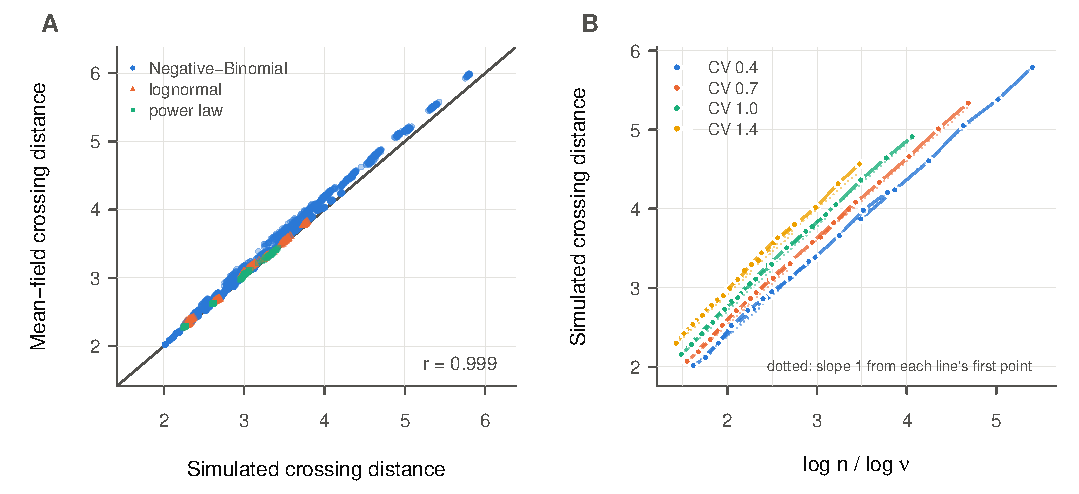
\includegraphics[width=0.9\linewidth]{figures/figureZ1_scaling.pdf}

\vspace{4pt}
\textbf{Figure 1. Mean-field prediction and scaling of the reversal distance in
configuration-model networks.} (A) Simulated against mean-field continuous
reversal distance for all 3{,}600 graphs, by degree family; the line is the
identity. (B) Mean simulated crossing against $\log n/\log\nu$ for the
Negative-Binomial cells, one line per (mean degree, CV) cell connecting its sizes;
the dotted segments have slope 1 and are drawn through each cell separately, because the intercept $c^*(p)$ differs between cells.
\end{figure*}

\subsection{Degree heterogeneity: an effect that changes sign with density}

Degree heterogeneity raises both the branching ratio $\nu$, which brings reversal
earlier, and the starting enrichment $1+\mathrm{CV}^2$, which delays it
(Section 4.4). Figure 2 shows the net effect, the change in the crossing when CV
rises from 0.4 to 1.4 at fixed size and mean degree. At mean degree 6 the crossing
falls by $0.5$ to $1.2$ steps, and at mean degree 12 by $0.03$ to $0.40$; at mean
degree 25 the change is $+0.22$ at $n=500$, $+0.13$ at $n=1{,}000$, and between
$-0.04$ and $+0.06$ for $n$ of 2{,}000 and more; at mean degree 50 and 100 it is
positive ($+0.04$ to $+0.29$ and $+0.13$ to $+0.30$). The mean degree at which the
effect changes sign rises with $n$. The mean-field model predicts exactly this
pattern (at $n=10^4$ the change over CV 0.4 to 2.0 is $-1.78$, $-0.71$, $-0.24$,
$-0.04$, $+0.17$, $+0.33$ for mean degrees 6, 12, 25, 50, 100, 200). Degree
heterogeneity therefore does not generally accelerate reversal; in sparse
networks it does, and in dense networks it delays it.

\begin{figure}[t]
\centering
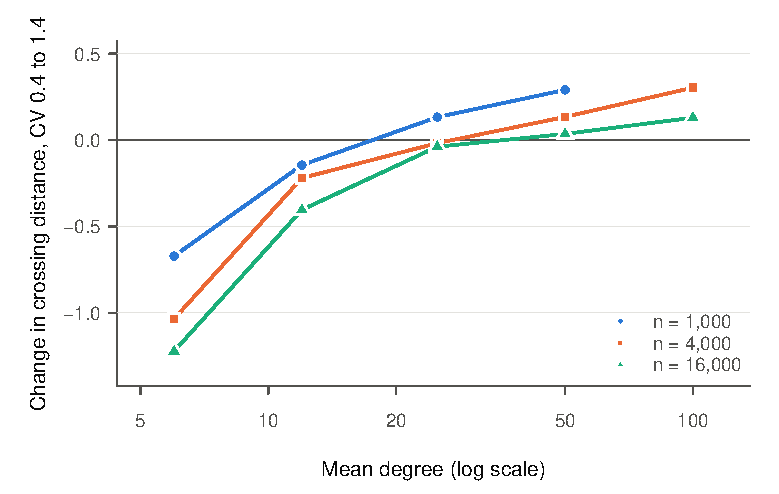
\includegraphics[width=0.78\linewidth]{figures/figureZ2_heterogeneity.pdf}

\vspace{4pt}
\textbf{Figure 2. The effect of degree heterogeneity on the reversal distance
depends on density.} Change in the mean continuous reversal distance when CV rises
from 0.4 to 1.4, at fixed size and mean degree (Negative-Binomial graphs).
\end{figure}

\section{Beyond the Degree Sequence: Assortativity, Clustering, and Communities}

\subsection{Design: exact control on fixed degree sequences}

Stage 2 starts from Negative-Binomial configuration-model graphs and rewires them
by degree-preserving double-edge swaps. We implemented the swaps with incremental
updates of the two quantities that change: with degrees fixed, assortativity changes
only through the sum of products of endpoint degrees over edges, and the global
clustering coefficient only through the triangle count. The routine accepts a swap if
it moves both quantities toward their targets, and it reproduces igraph's values of
both statistics on the rewired graphs. Targeting clustering alone drives
assortativity up (on a graph with 2{,}000 vertices and mean degree 25, a clustering
target of 0.30 moved assortativity from $-0.03$ to $0.71$), so we target both at once.
The two bases are (A) $n=2{,}000$, mean degree 25, CV 1.0 and (B) $n=4{,}000$, mean
degree 12, CV 1.4; assortativity targets are $-0.30,-0.15,0,0.15,0.30$ and clustering
targets the starting value, $0.10$, $0.20$, and $0.30$, with 30 graphs per cell
(1{,}200 graphs). Assortativity was within $0.002$ of its target and clustering
within $3\times10^{-4}$ in every graph.

\subsection{Clustering delays reversal; assortativity's effect depends on clustering}

Table 2 and Figure 3 give the results. Raising clustering from its starting value ($0.04$ in base A, $0.02$ in base B) to $0.30$ at zero assortativity delays reversal by $0.34$ steps in base A and $0.56$ in
base B. The effect of assortativity depends on clustering: at the starting
clustering, assortative wiring delays reversal (assortativity $+0.3$ against $-0.3$:
$+0.20$ and $+0.29$ steps), at clustering $0.10$ the effect is near zero, and at
clustering $0.20$ and above it is negative ($-0.16$ and $-0.15$ at $0.20$; $-0.07$
and $-0.30$ at $0.30$). The assortativity-by-clustering interaction in a regression
of the crossing is $-1.64$ (base A) and $-3.56$ (base B). Assortativity therefore
does not have a single sign in its effect on reversal. We do not have a mechanistic account of the sign change; the experiments establish it but do not explain it.

However, triangle-closing swaps also build community structure: modularity of the
detected partition rises by $0.34$ (base A) and $0.37$ (base B) between the
starting clustering and 0.30, mean distance rises by $0.16$ and $0.41$, and
clustering and modularity correlate $0.94$ and $0.93$ across graphs. In this
unrestricted rewiring clustering cannot be separated from community structure,
which motivates the next experiment.

\begin{figure*}[t]
\centering
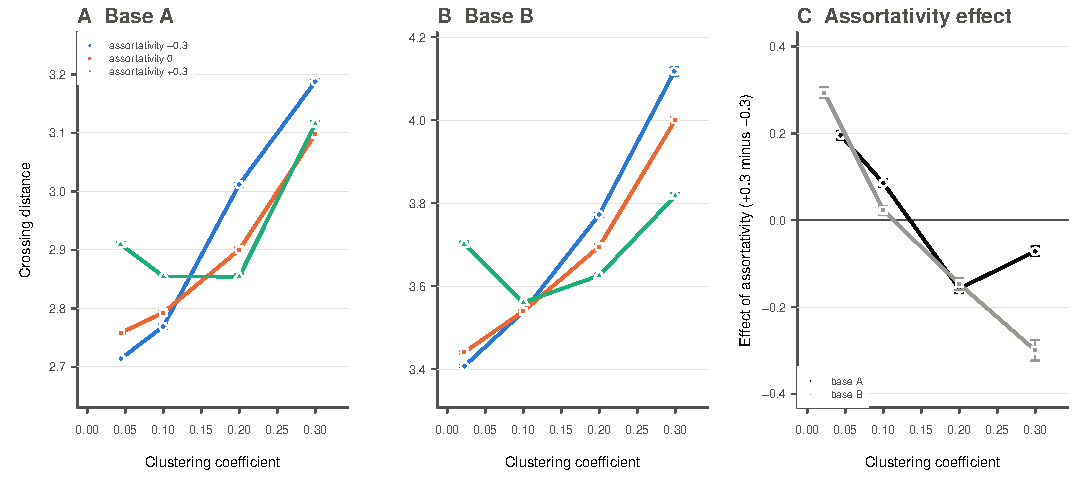
\includegraphics[width=0.95\linewidth]{figures/figureZ3_rewiring.pdf}

\vspace{4pt}
\textbf{Figure 3. Assortativity and clustering in rewired networks with fixed degree
sequences.} (A, B) Mean continuous reversal distance against the achieved
clustering coefficient for three assortativity targets, bases A and B ($\pm1$
standard error). (C) The effect of assortativity ($+0.3$ minus $-0.3$) on the
reversal distance by clustering, with 95\% intervals.
\end{figure*}

\subsection{Separating clustering from community structure}

To separate the two, we plant a partition of the vertices into blocks (10 blocks of
200 vertices in base A, 20 blocks of 200 in base B), draw each vertex's edges so
that a fraction $1-m$ stay within its block (mixing $m=0.15,0.30,0.50,0.80$,
corresponding to planted modularity $0.74$ to $0.17$ in base A and $0.79$ to $0.18$
in base B), and rewire with the additional rule that a swap is accepted only if it
leaves the number of edges between every pair of blocks unchanged. Then the planted
modularity, the degree sequence, and (to within $0.018$) assortativity are fixed
exactly while clustering is moved (960 graphs; 30 per cell). At weak community
structure the detected modularity still rises with the triangles (in base A with
$m=0.8$, from $0.17$ to $0.50$), so the separation is exact for the planted partition
and approximate for detected communities; at strong planted structure the detected
modularity hardly moves (base A, $m=0.15$: $0.74$ to $0.75$).

Both factors delay reversal (Table 2, Figure 4). Holding the planted communities
fixed, raising clustering across the range available in each cell (about $0.10$ to $0.30$
when communities are strong) delays reversal by $0.19$ to $0.28$ steps in base A and
$0.18$ to $0.64$ in base B (95\% intervals within $\pm0.02$ of these values). Holding clustering fixed at $0.10$, stronger communities (planted modularity
$0.74$ against $0.17$ in base A, $0.78$ against $0.18$ in base B) delay reversal
by $0.25$ and $0.28$ steps. The two effects have a positive interaction: the
effect of clustering is larger when communities are stronger. 
What the experiments establish is that these two rewiring procedures change the reversal
distance. The size of the change is easiest to read in whole steps: in the community experiments, in base A all 48
graphs in the lowest decile of clustering (mean $0.05$) reverse at distance 3 and all
48 in the highest decile (mean $0.30$) at distance 4, so a clustering difference of
about $0.25$ moves the reversal by one shell; in base B the highest decile splits between
distances 4 and 5 (15 and 33 graphs) while the lowest reverses at 4 in every graph.
A difference of $0.2$ to $0.3$ steps in the continuous measure is thus a visible fraction of the one-shell
step between neighbouring integer reversal distances, not a rounding artefact.

The data say less about why. The reversal distance tracks the mean distance of the
network very closely (correlation $0.994$), and when the mean distance is added to the regression the
coefficients of clustering and community strength shrink to near zero. Both are
summaries of the same distance distribution, so this does not show that mean
distance mediates the effect. A more direct check uses the shell profiles. In the
mean-field model enrichment is lost as the shells reach the hubs and then the rest of
the network. If wiring acts by slowing the expansion of the neighbourhoods, the fraction of the
network already reached at the crossing should vary much less than the crossing
distance does, and it does. Across all 3{,}600 configuration-model networks the cumulative share of
vertices within the crossing distance is $0.76$ on average (SD $0.06$) while the crossing distance itself
has SD $0.81$. In the controlled rewiring designs the share is $0.78$ (SD $0.02$) in base A and $0.69$
(SD $0.01$) in base B for the community experiments, and $0.78$ (SD $0.03$) and $0.70$ (SD $0.03$) for
the unrestricted rewiring, whereas an increase of $0.1$ in clustering moves the crossing by
$0.11$ to $0.20$ steps and the share at the crossing by only $0.01$ to $0.03$. This is what the saturation mechanism predicts: clustering and
communities delay the point at which the shells have covered about three quarters of the network.
Part of the regularity is forced, because the share must stay below one, so we read it as
consistent with the mechanism and not as a test that excludes other explanations. The first step of the expansion can be read directly: the ratio of the share of the network at distance 2 to the share at distance 1 falls by 14 to 24\% for each $0.1$ of clustering in the four designs. This is close to the definition of clustering (triangles leave fewer new vertices at distance 2) and so is expected, but it is the rate that the mean-field model takes as input.

\paragraph{Assortativity with the communities held fixed.} The sign change of Section 6.2 raises the question whether it arises because triangle-closing swaps also build communities, which assortative swaps then dissolve (in the unrestricted rewiring, at clustering $0.30$, detected modularity is lower by $0.20$ in base A and $0.24$ in base B at assortativity $+0.3$ than at $-0.3$). We therefore repeated the assortativity experiment inside the planted partitions, with block-pair edge counts fixed by the swap rule, three community strengths (mixing $0.15$, $0.5$, $0.8$), assortativity targets $-0.3$, $0$, $0.3$ (achieved to within $0.01$), and clustering either left at its natural value or raised to $0.20$ (1{,}080 graphs, 30 per cell; this experiment was added after the main analysis). Planted modularity and the degree sequence are exactly fixed. At natural clustering, raising assortativity from $-0.3$ to $+0.3$ delays reversal by $0.14$ (base A) and $0.21$ steps (base B), in each of the three community strengths. At clustering $0.20$ the effect falls to $-0.03$ and $+0.03$ (Table 2), with the six cells ranging from $-0.11$ to $+0.09$. The dependence on clustering therefore remains (the interaction is $-0.16$ and $-0.18$, $p<.001$), but its negative arm largely disappears: the clearly negative effects of $-0.16$ and $-0.15$ found with unrestricted rewiring at clustering $0.20$ are mostly the loss of community structure, and adjusting for detected modularity changes the interaction little ($-0.14$ and $-0.18$), so detected modularity is not the whole account. The remaining dependence is absorbed by the mean distance (to $-0.05$ and $-0.11$), which restates the result in terms of expansion and does not explain it.

\begin{table*}[t]
\centering
\textbf{Table 2.} Effects on the continuous reversal distance in rewired networks
with exactly fixed degree sequences (differences in means, 95\% intervals).

\vspace{4pt}
{\small\sf
\begin{tabular}{lrr}
\toprule
Contrast (condition) & Base A & Base B\\
\midrule
Clustering 0.30 vs start (assortativity 0) & $+0.340$ [0.327, 0.352] & $+0.560$ [0.545, 0.575]\\
Assortativity $+0.3$ vs $-0.3$ (start clustering) & $+0.196$ [0.186, 0.206] & $+0.294$ [0.281, 0.308]\\
Assortativity $+0.3$ vs $-0.3$ (clustering 0.10) & $+0.086$ [0.076, 0.095] & $+0.023$ [0.012, 0.033]\\
Assortativity $+0.3$ vs $-0.3$ (clustering 0.20) & $-0.158$ [$-0.168$, $-0.147$] & $-0.147$ [$-0.161$, $-0.133$]\\
Assortativity $+0.3$ vs $-0.3$ (clustering 0.30) & $-0.072$ [$-0.083$, $-0.060$] & $-0.300$ [$-0.324$, $-0.275$]\\
Clustering, highest vs lowest (planted modularity 0.60 / 0.63) & $+0.194$ [0.185, 0.203] & $+0.455$ [0.439, 0.471]\\
Clustering, highest vs lowest (planted modularity 0.74 / 0.78) & $+0.282$ [0.272, 0.293] & $+0.639$ [0.623, 0.655]\\
Community strength, strongest vs weakest (clustering 0.10) & $+0.248$ [0.238, 0.257] & $+0.278$ [0.267, 0.289]\\
Assortativity $+0.3$ vs $-0.3$ (planted partition fixed, natural clustering) & $+0.135$ [0.129, 0.141] & $+0.209$ [0.200, 0.217]\\
Assortativity $+0.3$ vs $-0.3$ (planted partition fixed, clustering 0.20) & $-0.028$ [$-0.033$, $-0.022$] & $+0.026$ [0.018, 0.035]\\
\bottomrule
\end{tabular}
\par}

\vspace{4pt}
{\small Base A: $n=2{,}000$, mean degree 25, CV 1.0; base B: $n=4{,}000$, mean degree 12,
CV 1.4; 30 graphs per cell. The first five rows are from unrestricted rewiring (1{,}200 graphs); the next three from rewiring that preserves the block-pair edge
counts of a planted partition (960 graphs); the last two from the same kind of rewiring with assortativity as the target (1{,}080 graphs, averaged over three community strengths, Section 6.3).}
\end{table*}

\begin{figure*}[t]
\centering
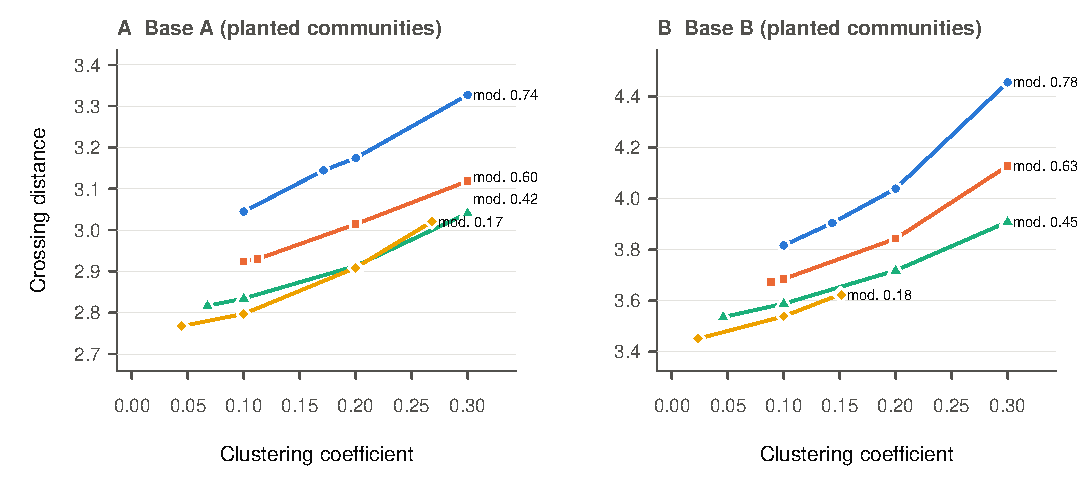
\includegraphics[width=0.9\linewidth]{figures/figureZ4_communities.pdf}

\vspace{4pt}
\textbf{Figure 4. Clustering at fixed planted community structure.} Mean continuous
reversal distance against the achieved clustering coefficient for four levels of
planted community strength ($Q$ is the planted modularity), bases A and B ($\pm1$
standard error). Rewiring preserves the number of edges between every pair of blocks.
\end{figure*}

\subsection{The first step: ego-averaged and pooled ratios, and assortativity}

Theorem 1(b) shows that the pooled first-step ratio depends
only on the degree distribution. The ego-averaged ratio does not: it also
depends on how degrees are correlated across edges.

\begin{proposition}[5 --- Ego-averaged ratio and assortativity]
Let $(D,D')$ be the degrees of the endpoints of a uniformly chosen edge, in a
uniformly random orientation, so that each has the size-biased marginal law
$\Lambda^*$. Then:
\begin{enumerate}
\item[(a)] The ego-averaged first-step ratio satisfies
$S_1^{\mathrm{ego}}:=A_1/\mu_1=\mathbb{E}[D/D']$ exactly, for any finite graph
without isolated vertices.
\item[(b)] $S_1^{\mathrm{ego}}-S_1=\mathrm{Cov}(D,1/D')$, where $S_1=\mu_2/\mu_1^2$
is the pooled value of Theorem 1(b).
\item[(c)] Fixing the marginal law $\Lambda^*$, $S_1^{\mathrm{ego}}$ is
antitone in the degree dependence of $(D,D')$ in the supermodular stochastic
order: it is maximal under the countermonotonic coupling (maximally
disassortative mixing) and minimal under the comonotonic coupling (maximally
assortative mixing), and under independent endpoint degrees
$S_1^{\mathrm{ego}}=S_1$.
\end{enumerate}
\end{proposition}

\begin{proof}
(a) $A_1=n^{-1}\sum_i d_i^{-1}\sum_{j\sim i}d_j$. Each edge $\{i,j\}$
contributes $d_j/d_i$ to $i$'s inner sum and $d_i/d_j$ to $j$'s, so
$\sum_i d_i^{-1}\sum_{j\sim i}d_j=\sum_{\{i,j\}\in E}(d_i/d_j+d_j/d_i)=2m\,
\mathbb{E}[D/D']$, where $m=|E|$ and we used that $(D,D')$ and $(D',D)$ have the same law.
Since $2m=n\mu_1$ we get $A_1=\mu_1\mathbb{E}[D/D']$.

(b) Under the size-biased marginal, $\mathbb{E}[D]=\mu_2/\mu_1$ and
$\mathbb{E}[1/D']=\sum_d d^{-1}(d\,p_d/\mu_1)=1/\mu_1$, so
$\mathbb{E}[D]\mathbb{E}[1/D']=\mu_2/\mu_1^2=S_1$. Hence
$S_1^{\mathrm{ego}}-S_1=\mathbb{E}[D/D']-\mathbb{E}[D]\mathbb{E}[1/D']=
\mathrm{Cov}(D,1/D')$.

(c) The function $f(d,d')=d/d'$ has mixed second difference
$f(d{+}1,d'{+}1)-f(d{+}1,d')-f(d,d'{+}1)+f(d,d')=-1/[d'(d'{+}1)]<0$, so $f$ is
strictly submodular. For two joint laws with the same marginals, the one that is
larger in the supermodular order yields a smaller $\mathbb{E}[f(D,D')]$ (Tchen,
1980; M\"uller \& Stoyan, 2002, Ch.~3). The comonotonic and countermonotonic
couplings are the maximum and minimum of that order among couplings with the
given marginals (Fr\'echet--Hoeffding bounds). Under independence, (b) gives
$\mathrm{Cov}(D,1/D')=0$.
\end{proof}

Newman's degree assortativity coefficient is the Pearson correlation of
$(D,D')$ on the same edge pairs, so part (b) says that for realistic joint
degree distributions positive assortativity lowers the ego-averaged ratio
below the pooled one, and negative assortativity raises it. We state the
result for $k=1$ only; for $k\ge2$ the corresponding dependence involves
longer-range degree correlations and we test it empirically.


\section{Empirical Networks}

\subsection{Data and approach}

We analyse Facebook friendship networks from 105 US universities (Traud, Mucha, \&
Porter, 2012), restricted to each network's largest component (762 to 63{,}392
vertices; mean degree 25.8 to 116.2; degree CV 0.71 to 1.55; clustering 0.10 to
0.29; assortativity $-0.07$ to $0.20$). For every network we compute $Q_k$ to the
diameter (all vertices for the 23 networks with at most 4{,}000 vertices, 2{,}000
sampled otherwise), the reversal distances with bootstrap standard errors, the
mean-field prediction from the degree sequence, the same quantities in a
degree-preserving randomisation (ten times as many swaps as edges), the modularity
of a Louvain partition, and the individual-level share $P_k$.

\subsection{How far away does the paradox reverse?}

The discrete reversal distance is 3 in 96 of the 105 networks (91\%), 4 in 8, and 5
in 1; because it varies so little we analyse the continuous reversal distance, which
has mean $2.75$ (SD $0.24$, range $2.23$ to $4.08$; bootstrap standard error at most
$0.017$). The mean enrichment is $Q_k=1.90$, $1.46$, $0.86$, $0.40$, $0.21$, and $0.11$ at $k=1,\ldots,6$ ($Q_1$ has SD $0.27$ and equals $1+\mathrm{CV}^2$ by Theorem 1(b)); $Q_2>1$ in every network, $Q_3<1$ in 91\%, and $Q_4<1$ in 99\%. The non-backtracking walk ratio of Section 2, by contrast, stays at its first-step level (mean ratios $1.71$, $1.04$, $1.03$ at steps 1 to 3, so the walk's endpoint has mean degree $1.71$, $1.78$, and $1.82$ times the population mean), as Proposition 2 says it does in the tree-like limit: a walk-based measure does not show the reversal that the neighbourhoods of a person undergo. On average 33\%, 55\%, 10\%, and 1\% of a network lies at distance 2, 3, 4,
and 5, and the share of people with a non-empty shell is 1.00 through $k=4$, 0.92 at
$k=5$, and 0.49 at $k=6$; the reversal therefore happens in shells that are large and
that every person has.

\subsection{Real networks reverse later than degree alone predicts}

Compare each network with two benchmarks that have its degree sequence and nothing
else (Figure 5A). A degree-preserving randomisation reverses earlier than the real
network in every one of the 105 networks, by $0.203$ steps on average (95\% interval
$[0.194,0.211]$; observed $2.75$, randomised $2.55$). The mean-field model, which
sees only the degree sequence, matches the randomised networks closely (correlation
$0.999$, mean-field later by $0.02$ steps) and so it also reverses earlier than the real
networks (correlation with the observed crossing $0.982$, root-mean-square
difference $0.19$, mean-field earlier by $0.18$). The offset is therefore not an error
of the model: it is a property of how real networks are wired.

\subsection{What explains the offset?}

Table 3 reports regressions across the 105 networks. The reversal distance falls
with mean degree and rises with size, as in the simulations, and it is higher in
networks with more assortative mixing ($+0.65$ per unit of assortativity,
$p<.001$), more clustering ($+0.94$, $p=.017$), and more heterogeneous degrees
($+0.17$, $p=.016$), with $R^2=0.94$. Adding the modularity of a detected partition
raises $R^2$ to $0.96$; modularity has a large coefficient ($+1.06$, $p<.001$) and
clustering's coefficient falls to $+0.39$ ($p=.21$). Clustering is strongly
collinear with log size ($r=-0.87$; variance inflation factors 5.3 for clustering and
8.2 for log size), so its coefficient is the least reliable in the table. The
departure from the mean-field prediction, the observed minus the mean-field
crossing, is accounted for by assortativity ($+0.47$ per unit, $p<.001$) and
modularity ($+0.85$, $p<.001$), with clustering, CV, size, and mean degree not
significant ($R^2=0.71$; $0.69$ with assortativity and modularity alone;
Figure 5B). The experiments of Section 6 suggest the same for community structure, which delays reversal when added to a fixed degree sequence. For assortativity the experiments show that the sign of the effect depends on clustering, so the cross-sectional coefficient describes these networks and is not a replication of a single effect. The Facebook networks have clustering between $0.10$ and $0.29$ (83\% between $0.10$ and $0.20$), which is the range in which Table 2 finds the effect of assortativity changing from small positive to negative. The cross-sectional association of the offset with assortativity is nevertheless positive in each third of the clustering distribution (slopes $0.32$ to $0.66$) and shows no interaction with clustering ($p=.95$). This is more consistent with the experiments than it first appears. With the communities held fixed (Section 6.3) the experimental effect of assortativity is positive at natural clustering ($+0.14$ and $+0.21$ for a change of $0.6$ in assortativity, a slope of $0.2$ to $0.35$ per unit) and close to zero at clustering $0.20$, not clearly negative, and the Facebook networks' assortativity spans only $-0.07$ to $0.20$. The cross-sectional slope ($0.32$ to $0.66$ per unit) is larger than the experimental one, so the cross-section carries more than degree mixing alone: assortativity is tied to other features of the networks, for instance the mixing of students by year, which we have not separated.

The cross-sectional slope of the crossing on
$\log n/\log\nu$ is $1.43$ ($R^2=0.93$); since the degree law varies across networks
this is not a test of the translation property. The mean-field crossings for the same networks have
slope $1.31$, so most of the excess over $1$ comes from the variation of $c^*(p)$ with the degree law and not from
anything particular to real networks.

\begin{table*}[t]
\centering
\textbf{Table 3.} Regression of the continuous reversal distance, and of its
departure from the mean-field prediction, on network features (105 Facebook networks).

\vspace{4pt}
{\small\sf
\begin{tabular}{lrrr}
\toprule
Predictor & Reversal distance & Reversal distance (with modularity) & Observed $-$ mean-field\\
\midrule
Intercept & 0.619** (0.194) & 0.578*** (0.153) & $-0.221$* (0.086)\\
Degree CV & 0.172* (0.070) & 0.257*** (0.056) & 0.053 (0.032)\\
Assortativity & 0.649*** (0.125) & 0.783*** (0.099) & 0.471*** (0.056)\\
Clustering & 0.944* (0.391) & 0.394 (0.315) & 0.092 (0.178)\\
Mean degree (per 10) & $-0.063$*** (0.004) & $-0.054$*** (0.003) & 0.003 (0.002)\\
log(N) & 0.247*** (0.017) & 0.193*** (0.015) & $-0.011$ (0.009)\\
Modularity (Louvain) & --- & 1.056*** (0.134) & 0.847*** (0.076)\\
$R^2$ & 0.940 & 0.963 & 0.713\\
\bottomrule
\end{tabular}
\par}

\vspace{4pt}
{\small *$p<.05$, **$p<.01$, ***$p<.001$. OLS; standard errors in parentheses. Degree CV
$=\mathrm{SD}/\mathrm{mean}$ of degree; assortativity is Newman's (2002) coefficient;
clustering is the global clustering coefficient. Variance inflation factors in the
second column: clustering 5.3, log size 8.2, others below 2.6. $N=105$.}
\end{table*}

\begin{figure*}[t]
\centering
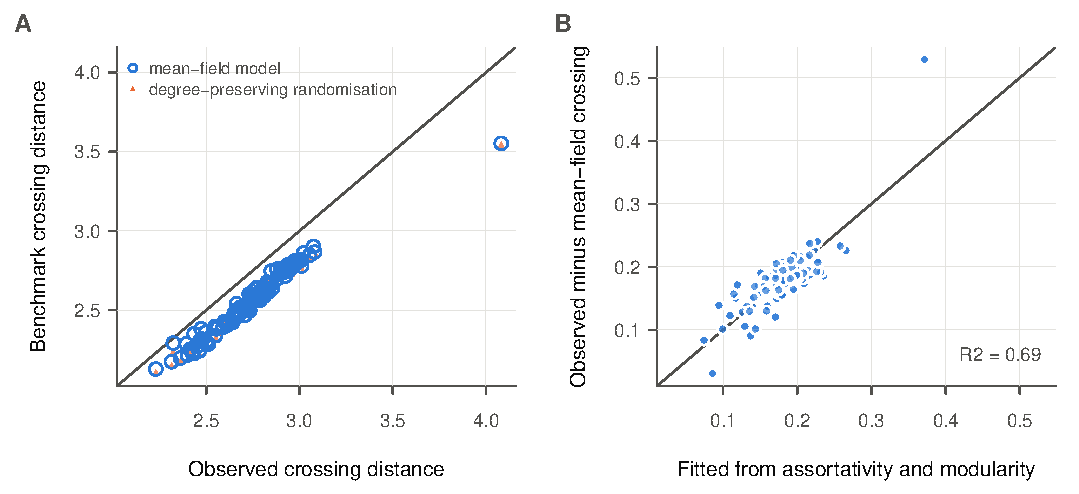
\includegraphics[width=0.9\linewidth]{figures/figureZ5_facebook.pdf}

\vspace{4pt}
\textbf{Figure 5. Reversal distance in 105 Facebook networks.} (A) The continuous
reversal distance predicted by the mean-field model (blue) and found in a
degree-preserving randomisation (orange), against the observed value; the line is the
identity. (B) The observed minus the mean-field crossing against its fitted value from
a regression on assortativity and modularity ($R^2=0.69$).
\end{figure*}

\subsection{Networks of other kinds}

Facebook university networks are dense, with small diameters, and the model predicts
that reversal comes later in larger and sparser networks. We therefore applied the
same analysis to ten public networks from the Stanford Network Analysis Project
collection (Leskovec \& Krevl, 2014), chosen to differ in size, density, and kind:
four scientific collaboration networks (arXiv GrQc, HepTh, CondMat, AstroPh;
Leskovec, Kleinberg, \& Faloutsos, 2007), the Enron email network (Klimt \& Yang, 2004; Leskovec, Lang, Dasgupta, \& Mahoney, 2009), a Facebook ego
network (McAuley \& Leskovec, 2012), two location-based social networks (Brightkite
and Gowalla; Cho, Myers, \& Leskovec, 2011), and two large networks from
Yang and Leskovec (2015), an Amazon co-purchase network (335{,}000 vertices) and the
DBLP collaboration network (317{,}000 vertices). Edge lists were read as undirected
simple graphs and restricted to their largest components (4{,}039 to 334{,}863
vertices; mean degree 5.5 to 43.7; Table 4). The computations are those of
Section 7.1, with 2{,}000 sampled start vertices where $n>4{,}000$.

All ten networks reverse, and at distances that are much larger than in the Facebook
networks: the continuous reversal distance runs from $3.71$ (Enron) to $11.36$
(Amazon), against a Facebook mean of $2.75$, and the diameters seen run from 8 to 46
(bootstrap standard errors at most $0.043$). The degree-sequence benchmarks
follow $\log n/\log\nu$ closely (correlation $0.97$ for the randomised networks and
$0.98$ for the mean-field model; the observed crossing, $0.92$), so large and sparse
networks do reverse later, as predicted. The mean-field model again matches the
degree-preserving randomisations (correlation $0.999$; the largest difference is $0.11$
steps), and again the real networks reverse later than both, in every one of the ten
networks, by $0.27$ to $5.10$ steps (mean $1.32$; Figure 6A). The offset is much larger
than in the Facebook networks, and it is ordered by community structure: the
observed minus mean-field crossing has a Spearman correlation of $0.99$ and a
Pearson correlation of $0.79$ with modularity across the ten networks, and $0.75$ across
all 115 networks (Figure 6B). It is $0.23$ in the Enron email network (modularity $0.59$),
about $1$ to $1.7$ in the collaboration networks and the ego network (modularity $0.76$ to $0.85$),
and $5.1$ in the Amazon co-purchase network (modularity $0.93$). Dropping any one network leaves the Spearman correlation between $0.98$ and $1.00$, and the Pearson correlation between $0.78$ and $0.93$ (it is highest without the Amazon network). Clustering and assortativity
are weakly related to the offset in these ten ($r=0.15$ and $-0.06$), which with ten networks is not informative. The slope of the observed crossing on $\log n/\log\nu$ in these ten is $1.86$, against $0.92$ for the mean-field crossings; the difference is the offset. The
individual-level crossing lags the reversal distance by $0.74$ to $4.84$ steps (mean $1.69$;
correlation $0.99$), so the paradox lasts longer for the less connected in these networks
as well, and by a wider margin where reversal is late. These are ten networks from
one repository, selected for variety and not sampled; we regard this as a test that the
predictions of Section 4 and the Facebook findings are not particular to
Facebook-type networks, not as an estimate of any population quantity. For the same reason the modularity ordering of the offset in these ten is a consistency check on the Facebook result, which has the power to estimate the effect, and not an independent estimate of it.

\begin{table*}[t]
\centering
\textbf{Table 4.} Reversal distance in ten public networks (largest components).

\vspace{4pt}
{\small\sf
\begin{tabular}{lrrrrrrrrr}
\toprule
Network & $n$ & Mean deg. & CV & Clust. & Assort. & Modul. & Observed & Randomised & Mean-field\\
\midrule
Enron email & 33{,}696 & 10.7 & 3.50 & 0.09 & $-0.12$ & 0.59 & 3.71 & 3.44 & 3.48\\
AstroPh & 17{,}903 & 22.0 & 1.41 & 0.32 & 0.20 & 0.62 & 3.92 & 3.30 & 3.33\\
Brightkite & 56{,}739 & 7.5 & 2.74 & 0.11 & 0.01 & 0.68 & 4.55 & 3.94 & 3.94\\
Gowalla & 196{,}591 & 9.7 & 5.54 & 0.02 & $-0.03$ & 0.71 & 4.27 & 3.78 & 3.68\\
CondMat & 21{,}363 & 8.5 & 1.28 & 0.26 & 0.13 & 0.72 & 4.98 & 4.16 & 4.21\\
HepTh & 8{,}638 & 5.7 & 1.12 & 0.28 & 0.24 & 0.76 & 5.56 & 4.60 & 4.68\\
DBLP & 317{,}080 & 6.6 & 1.51 & 0.31 & 0.27 & 0.82 & 6.33 & 5.22 & 5.25\\
Facebook ego & 4{,}039 & 43.7 & 1.20 & 0.52 & 0.06 & 0.83 & 4.00 & 2.58 & 2.62\\
GrQc & 4{,}158 & 6.5 & 1.34 & 0.63 & 0.64 & 0.85 & 5.66 & 3.89 & 3.96\\
Amazon co-purchase & 334{,}863 & 5.5 & 1.04 & 0.21 & $-0.06$ & 0.93 & 11.36 & 6.26 & 6.30\\
\bottomrule
\end{tabular}
\par}

\vspace{4pt}
{\small Note: Clust. is the global clustering coefficient, Assort. Newman's degree
assortativity, Modul. the modularity of a Louvain partition. The last three columns are
the continuous reversal distance of the network, of a degree-preserving
randomisation, and of the mean-field model. Ordered by modularity.}
\end{table*}

\begin{figure*}[t]
\centering
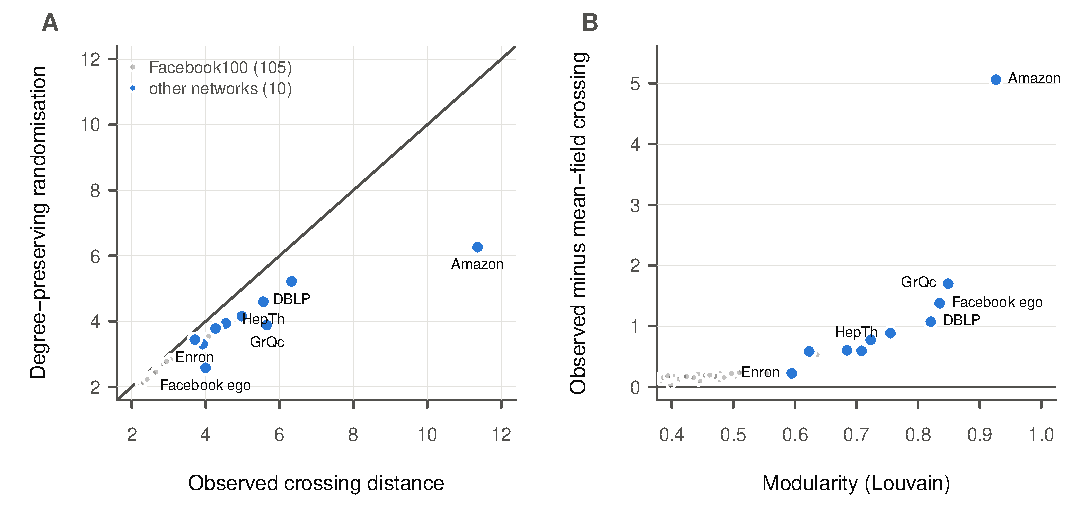
\includegraphics[width=0.9\linewidth]{figures/figureZ6_external.pdf}

\vspace{4pt}
\textbf{Figure 6. Reversal distance in ten public networks and in the Facebook
networks.} (A) Reversal distance of a degree-preserving randomisation against the
observed value (identity line). (B) The observed minus the mean-field crossing against
modularity. Facebook100 networks in grey, the ten other networks in blue.
\end{figure*}

\section{For Whom Does the Paradox Last?}

The reversal distance describes the average person at distance $k$. Feld's paradox
compares a person with their own friends, so we also ask how many people still
experience it at distance $k$: the share $P_k$ of people whose distance-$k$ shell has
a higher mean degree than their own degree. Averaged over the 105 networks, $P_k$ is
85\%, 75\%, 50\%, 17\%, and 5\% at $k=1,\ldots,5$ (Table 5). A majority of people have
the paradox at distance 2 in every network, at distance 3 in 53 of the 105 networks,
and at distance 4 in one. It depends strongly on one's own degree (Figure 7): for the
third of people with the lowest degree in each network, the paradox holds for
essentially all of them through distance 3 and for half at distance 4; for the middle
third it holds through distance 2 and for half at distance 3; for the highest third it
holds for 57\% at distance 1 and for 25\% at distance 2, and is absent beyond.
Proposition 4 explains the form of this result in the model: for $k=1,2$ the paradox
holds exactly for people below a threshold degree, and the threshold falls with
distance. The mean-field model tracks the shares across networks (correlations
$0.97$ to $0.98$ at $k=1,\ldots,4$, root-mean-square errors $0.01$ to $0.09$),
underpredicting $P_3$ and $P_4$ by $0.08$.

The individual-level crossing, the distance at which $P_k$ falls through one half,
follows the reversal distance closely. In the Facebook networks it lies $0.24$ steps
later (SD $0.06$; correlation $0.99$); in the 3{,}600 simulated networks $0.28$ steps
later (SD $0.15$; correlation $0.98$); and in the mean-field model $0.2$ to $0.35$
steps later at every size we tried. For the less connected the paradox therefore lasts a little
longer than the population-level reversal suggests.

\begin{table}[t]
\centering
\textbf{Table 5.} Share of people with the paradox at distance $k$ (105 Facebook networks).

\vspace{4pt}
{\small\sf
\begin{tabular}{rrrrr}
\toprule
$k$ & Observed mean (SD) & Range & Mean-field mean & Share with $B_k>\mu_1$\\
\midrule
1 & 0.85 (0.03) & 0.79--0.94 & 0.85 & 0.89\\
2 & 0.75 (0.05) & 0.63--0.92 & 0.73 & 0.98\\
3 & 0.50 (0.08) & 0.30--0.84 & 0.43 & 0.28\\
4 & 0.17 (0.07) & 0.05--0.66 & 0.09 & 0.02\\
5 & 0.05 (0.04) & 0.01--0.40 & --- & 0.00\\
\bottomrule
\end{tabular}
\par}

\vspace{4pt}
{\small Note: the share of people whose distance-$k$ shell has a higher mean degree
than their own degree; the last column is the share whose shell mean exceeds the
population mean degree.}
\end{table}

\begin{figure*}[t]
\centering
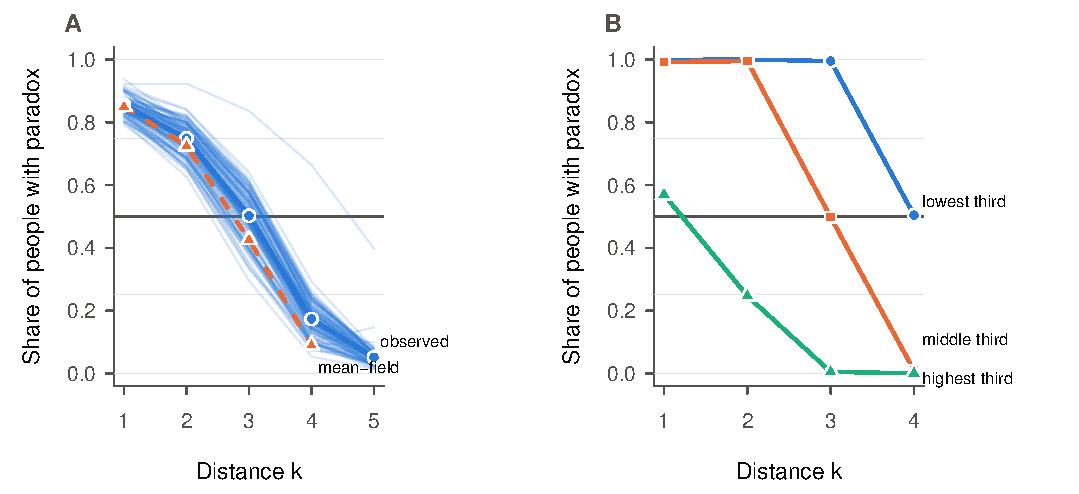
\includegraphics[width=0.9\linewidth]{figures/figure4_individual.pdf}

\vspace{4pt}
\textbf{Figure 7. The paradox at the level of the individual.} (A) Share of people
whose distance-$k$ shell has a higher mean degree than their own degree, one thin
line per network, the mean in bold, and the mean-field prediction (orange, dashed); the horizontal line is one half.
(B) The same share by a person's own degree (thirds of the degree distribution
within each network, averaged over networks).
\end{figure*}

\section{Discussion and Conclusion}

The friendship paradox must reverse in every finite connected network that is not regular,
because degrees average to the population mean. The distance of reversal, which the
argument does not fix, is predictable from the degree distribution and shifted by wiring. In a mean-field model of hub-first
saturation the reversal distance grows as $\log n/\log\nu$ plus a term set by the
degree law, an exact translation property of the model; in 3{,}600 simulated networks
the model predicts the reversal distance with a correlation of $0.999$, and mean
degree and size act as the model predicts, while the effect of degree heterogeneity
changes sign with density: in sparse networks it brings reversal earlier, in dense
ones it delays it. Beyond the degree sequence, clustering and community structure
each delay reversal and have a positive interaction, and assortativity's effect
depends on clustering. In the 105 Facebook networks reversal comes about $0.2$ steps later than in degree-preserving randomisations in every network, and assortativity and modularity account for most of that offset; in ten other networks the offset is larger, up to $5$ steps, and is ordered by modularity. For individuals the paradox lasts
longest for the least connected.

For the higher-order paradox the results mean the following. The answer to
``does a person's friends-of-friends have more friends than the person?'' is
yes for most people at distance 2 and for about half at distance 3 in these networks,
and the population-level answer, that the people at distance 3 are less connected
than average, is true of most of the networks; but the distance at which this
happens is not constant. It moves with the size, density, and wiring of the network
in the way the model describes, and a longer chain of acquaintance is needed in larger
and sparser networks.

The study has limits. The scaling result is proved for the mean-field model; for graphs it is an
empirical statement, accurate to about $\pm0.15$ in the slope at the sizes we simulated, and it has been tested only within configuration-model degree laws, where the model's assumptions hold by construction. Outside them, in the empirical networks, we compare the observed crossing with the model's prediction and find an offset; we have no separate test of the scaling there. The individual-level result (the paradox lasts longest for the least connected) is proved in the model for $k\le2$ and is an empirical finding beyond that.

The simulations use two bases, a Negative-Binomial degree law, and equal-sized planted
blocks; assortativity and clustering are manipulated with greedy swaps, and the
separation of clustering from communities is exact for the planted partition and
approximate for detected communities.

The reversal distance is almost a function of
the mean distance of the network, and the share of the network reached at the crossing
varies little across conditions; both are consistent with clustering and community
structure acting by slowing the expansion of neighbourhoods, but both are summaries of the
same distance distribution and do not establish mediation.

The analysis plan was written before the Stage 1 and Stage 2 data were analysed and is kept with the code, not registered externally. Three analyses were added after the main analysis (the shell-coverage diagnostic, the assortativity experiment inside planted partitions, and the numerical checks of the proofs), and the pooled slope test for the power-law family departs from its pre-specified form; the replication materials list each hypothesis, its outcome, and these departures.

The three kinds of evidence differ in what they support. The simulations establish controlled results within the stated generating and rewiring procedures; the Facebook networks show that the same patterns hold consistently in one family of related networks, not 105 independent draws from a population of social networks; and the ten other networks show that the patterns are not confined to Facebook, not that they are universal.

The empirical analysis rests mainly on one class of networks, university Facebook networks, which are dense and have small diameters; ten public networks of other kinds, from one repository and chosen for variety, show reversal at larger distances (up to $11$ steps) as the model predicts for large and sparse networks, but they are too few to support more than that. In the Facebook data clustering is collinear with size, and
regressions of 105 correlated networks are associations. Finally, the analysis
concerns degree; the same question can be asked of any node attribute.

The results have a practical reading for sampling. A random-walk-based sample
reaches vertices whose degree is size-biased at every step, whereas a design that
collects everyone within distance $k$ collects, from the reversal distance onward,
people with lower degree than average; and the reversal distance is later in larger,
sparser, and more modular networks. The choice of design, and how
far one goes, determines the sign of the bias. A sampler who wants a degree-representative sample should therefore not collect whole shells beyond the reversal distance, which oversamples low-degree people, and should not use random-walk steps, which oversample high-degree people at every step; the reversal distance tells how far a shell-based design can go before the bias changes sign.


\section*{Data and Code Availability}

The Facebook100 networks are publicly available (Traud, Mucha, \& Porter, 2012), as are the ten additional networks (Stanford Network Analysis Project; Leskovec \& Krevl, 2014). All simulation and analysis code, the derived results behind every table and figure, and the analysis plan are available at https://anonymous.4open.science/r/33CC/ (anonymised for review).

\appendix

\section{Proof of Proposition 3}

\textbf{Roadmap.} (1) The exposure of a start vertex obeys a one-dimensional map $E_{k+1}=\delta_s+H(E_k)$ in which $n$ enters only through $\delta_s$ (Section 4.3). (2) Without the constant, $H$ has a repelling fixed point at $0$ with multiplier $\nu$; Koenigs' theorem for the inverse branch gives a Poincar\'e function $\omega$ with $H(\omega(u))=\omega(\nu u)$, which is the $n$-free curve that all orbits follow. (3) Lemma A shows that the orbit of the map with the constant follows $\omega$ at the scale $\nu^k\delta_s/(\nu-1)$: a linear phase while the exposure is small, then a nonlinear phase in which $H$ is $\nu$-Lipschitz. (4) Substituting into the enrichment gives $\mathcal Q$ and the translation property. (5) The reversal distance is read off from where $\mathcal Q$ crosses $1$, with a separate argument when the crossing falls close to a shell. The steps are independent: a reader who accepts Lemma A can check (4) and (5) from the displayed formulas.

\textbf{Poincar\'e function and the limit profile.} $H$ is increasing and strictly concave with $H(0)=0$, $H'(0)=\nu>1$,
and has a unique fixed point $E^*\in(0,1)$. Koenigs' linearisation theorem (Milnor, 2006, Theorem 8.2), applied to the inverse branch of $H$ at $0$, which is attracting (as in Milnor's own treatment of the repelling case; details below), gives an
increasing analytic bijection $\omega:[0,\infty)\to[0,E^*)$ with $\omega(u)=u+O(u^2)$ and $H(\omega(u))=\omega(\nu u)$, and
the orbit of \eqref{eq:onedim} tracks $\omega$ along the scale $\nu^k\delta_s/(\nu-1)$ (Lemma A below). Define, for $\lambda>0$,
\begin{equation*}
\mathcal Q(\lambda)=\frac{\sum_s p_s\sum_d p_d\,d\,\bigl(e^{-d\,\omega(\lambda s/(\nu\kappa))}-e^{-d\,\omega(\lambda s/\kappa)}\bigr)}
{\mu_1\sum_s p_s\sum_d p_d\,\bigl(e^{-d\,\omega(\lambda s/(\nu\kappa))}-e^{-d\,\omega(\lambda s/\kappa)}\bigr)},\qquad \kappa=\mu_1(\nu-1).
\end{equation*}
\textbf{Periodic correction.} With $g(t)=\mathcal Q(\lambda^*\nu^t)$ and $\{u\}$ the fractional part,
\begin{equation*}
\pi(u)=-\{u\}+\frac{g(-\{u\})-1}{g(-\{u\})-g(1-\{u\})},
\end{equation*}
which is continuous and $1$-periodic with $\pi(0)=0$. Numerically, $\mathcal Q$ reproduces the mean-field enrichment to $4\times10^{-4}$ at $n=10^3$ and
$2\times10^{-7}$ at $n=10^7$ (Negative-Binomial degrees, mean degree 12, CV 1.0), and the continuous reversal distance differs from
$\log_\nu(n\lambda^*)$ by at most $0.016$ ($\lambda^*=13.35$, $c^*=0.83$ for that law).

\textbf{One-dimensional reduction.} This is derived in Section 4.3: with
$H(E)=\mu_1^{-1}\sum_dp_d(d-1)(1-e^{-dE})$ the exposure of a start vertex of degree
$s$ is the orbit of $\psi_\delta(E)=\delta+H(E)$ from $E_0=0$, $\delta=\delta_s=s/(n\mu_1)$,
and the mean-field enrichment is
\begin{equation*}
\tilde Q_k(n)=\frac{\sum_s p_s\sum_d p_d\,d\,\pi_k(d\mid s)}{\mu_1\sum_s p_s\sum_d p_d\,\pi_k(d\mid s)},\qquad
\pi_k(d\mid s)=e^{-dE_{k-1}(s)}-e^{-dE_k(s)} .
\end{equation*}

\textbf{Properties of $H$.} $H$ is analytic, $H'(E)=\mu_1^{-1}\sum_dp_d\,d(d-1)e^{-dE}>0$ is
decreasing (so $H$ is strictly concave; some $d\ge2$ has $p_d>0$ since $\nu>1$),
$H'(0)=\nu$, and $H(E)\le1-1/\mu_1<1$. Concavity makes $H(E)/E$ decreasing, so
$H(E)>E$ exactly on $(0,E^*)$ for a unique fixed point $E^*\in(0,1)$ with
$H'(E^*)<1$. Let $h$ be the inverse branch of $H$ near $0$; it is analytic with
$h'(0)=1/\nu<1$. By Koenigs' theorem (Milnor, 2006, Theorem 8.2) the limit
$\varphi(E)=\lim_k\nu^kh^k(E)$ exists, is analytic near $0$ with $\varphi(E)=E+O(E^2)$,
and satisfies $\varphi(H(E))=\nu\varphi(E)$. Since $h^k(E)\to0$ for every
$E\in(0,E^*)$ and $h$ is increasing, $\varphi$ extends to an increasing bijection
$[0,E^*)\to[0,\infty)$ (it diverges at $E^*$ because $E^*$ is repelling for $h$) with
the same functional equation; $\omega=\varphi^{-1}$ is the Poincar\'e function. Two details: $H$ maps $[0,E^*)$ bijectively onto itself, so $h$ is defined on $[0,E^*)$ with $h(E)<E$, and its only fixed point there is $0$. If $\varphi(E)\to L<\infty$ as $E\uparrow E^*$, then $\varphi(H(E))=\nu\varphi(E)$ gives $L=\nu L$, so $L=0$ or $\infty$; $L=0$ is impossible because $\varphi>0$ on $(0,E^*)$, which proves the divergence. Differentiating, $\varphi'(H(E))H'(E)=\nu\varphi'(E)$ with $\varphi'(0)=1$ and $H'>0$ shows $\varphi'>0$, so $\omega$ is analytic and Lipschitz on compact sets. The orbit of $\psi_\delta$ settles at the fixed point $E^*_\delta>E^*$ of $\psi_\delta$, which tends to $E^*$ as $\delta\to0$; Lemma A only concerns the part of the orbit with bounded $\nu^k\delta$, before it settles.

\textbf{Lemma A.} Let $\delta>0$ and $E_k=E_k(\delta)$ be the orbit of $\psi_\delta$ from $0$.
For every $0<a<b<\infty$,
$\sup\{|E_k-\omega(\nu^k\delta/(\nu-1))|:\ \nu^k\delta/(\nu-1)\in[a,b]\}\to0$ as $\delta\to0$.

\emph{Proof.} The orbit is increasing and stays below the fixed point of $\psi_\delta$.
\emph{Linear phase.} Concavity gives $H(E)\le\nu E$, so $E_k\le\delta\nu^k/(\nu-1)$
for all $k$. Choose $C$ and $E_0$ with $H(E)\ge\nu E-CE^2$ for $E\le E_0$, and let
$0<\eta\le E_0$. With $z_k=\nu^{-k}E_k$ we have
$z_{k+1}-z_k=\delta\nu^{-(k+1)}-\nu^{-(k+1)}\bigl(\nu E_k-H(E_k)\bigr)$, where
$0\le\nu E_k-H(E_k)\le CE_k^2$ while $E_k\le E_0$. Summing and using the upper bound,
\[
\frac{\delta}{\nu-1}\bigl(1-\nu^{-k}\bigr)-C_1\delta^2\nu^{k}\;\le\;z_k\;\le\;\frac{\delta}{\nu-1}\bigl(1-\nu^{-k}\bigr)
\]
for every $k$ with $E_k\le E_0$. Let $K$ be the first $k$ with $E_k\ge\eta$. The lower
bound shows that $E_k\ge\nu^k\delta/(2(\nu-1))$ whenever $y_k:=\nu^k\delta\le y_0$ (for a suitable $y_0>0$) and $k$ is large. Let $k_0$ be the last $k$ with $y_k\le y_0$; then $y_{k_0}>y_0/\nu$, so $E_{k_0}>y_0/(2\nu(\nu-1))>\eta$ for $\eta$ small, hence $K-1\le k_0$ and the bound applies at $K-1$. Therefore $K\to\infty$ and $\delta\nu^K\le2\nu(\nu-1)\eta$ for small $\eta$ and
$\delta$; then $C_1\delta^2\nu^K\le C_2\delta\eta$ and
\[
E_K=\frac{\nu^K\delta}{\nu-1}(1+\theta),\qquad |\theta|\le C_3\eta+o(1),\qquad \eta\le E_K\le\nu\eta+\delta .
\]
\emph{Nonlinear phase.} Since $\psi_\delta=H+\delta$ and $H$ is $\nu$-Lipschitz,
$|E_{K+j}-H^j(E_K)|\le\delta(\nu^j-1)/(\nu-1)$. Take $\eta<a/(2\nu)$, so that $k\ge K$ for every $k$ with $\nu^k\delta/(\nu-1)\in[a,b]$ once $\delta$ is small. Any $k$ with
$\nu^k\delta/(\nu-1)\in[a,b]$ equals $K+j$ with $0\le j\le J:=\log_\nu(b/\eta)+2$,
a bound that does not depend on $\delta$. Therefore $E_{K+j}=H^j(E_K)+O(\delta\nu^J)$,
and $H^j(E_K)=\omega\bigl(\nu^j\varphi(E_K)\bigr)=\omega\bigl(\nu^{K+j}\delta(1+\theta')/(\nu-1)\bigr)$
with $|\theta'|\le C_4\eta+o(1)$, because $\varphi(E)=E(1+O(E))$ and $E_K\le\nu\eta+\delta$.
As $\omega$ is Lipschitz on compact sets with constant $L$,
$|E_k-\omega(\nu^k\delta/(\nu-1))|\le L\,C_4\,b\,\eta+O(\delta\nu^J)+o(1)$.
Letting $\delta\to0$ and then $\eta\to0$ proves the lemma. \qed

\textbf{Proof of Proposition 3.} For each of the finitely many start degrees $s$,
$\delta_s=s/(n\mu_1)$, so $\nu^k\delta_s/(\nu-1)=\lambda s/\kappa$ with
$\lambda=\nu^k/n$ and $\kappa=\mu_1(\nu-1)$; the same holds for $k-1$ with
$\lambda/\nu$. By Lemma A, uniformly over $k$ with $\nu^k/n\in\Lambda$ compact, both
$E_{k-1}(s)$ and $E_k(s)$ are within $o(1)$ of $\omega(\lambda s/(\nu\kappa))$ and
$\omega(\lambda s/\kappa)$. $\tilde Q_k(n)$ is a continuous function of these
finitely many numbers whose denominator is bounded away from zero on $\Lambda$, so
$\tilde Q_k(n)=\mathcal Q(\nu^k/n)+o(1)$, uniformly. Replacing $(k,n)$ by
$(k+1,\nu n)$ leaves $\nu^k/n$ unchanged, so $\tilde Q_{k+1}(\nu n)-\tilde Q_k(n)\to0$.
For $\lambda\to0$ all exposures are small, $\pi_k(d\mid s)=d\,x_k(s)(1+O(d\,E_k))$ with
$x_k(s)\propto s$, and the ratio tends to $\mu_2/\mu_1^2$ (this also gives
$\tilde Q_k(n)>1$ uniformly for $\nu^k/n$ small enough). For the reversal distance, write $g(t)=\mathcal Q(\lambda^*\nu^t)$.
By hypothesis $g>1$ on $t<0$ and $g<1$ on $(0,1]$, and $g(0)=1$ by continuity. Fix $\varepsilon>0$.
Since $\mathcal Q\to\mu_2/\mu_1^2>1$ as $\lambda\to0$ and $\mathcal Q$ is continuous, $\mathcal Q\ge1+\eta$ on
$(0,\lambda^*\nu^{-\varepsilon}]$ for some $\eta>0$, and $\mathcal Q\le1-\eta$ on $[\lambda^*\nu^{\varepsilon},\nu\lambda^*]$.
The uniform convergence on compacts, together with the uniform lower bound for small $\nu^k/n$, therefore gives
that for large $n$, $\tilde Q_k(n)>1$ whenever $k-u(n)\le-\varepsilon$ and $\tilde Q_k(n)<1$ whenever
$k-u(n)\in[\varepsilon,1]$. If $u$ is at least $\varepsilon$ from an integer, the first shell below $1$ is therefore
$\lfloor u\rfloor+1=\lceil u\rceil$. If $u$ is within $\varepsilon$ of an integer $m$, shells up to $m-1$ lie above $1$,
and shell $m+1$ lies below $1$ (it is at $k-u\ge1-\varepsilon$ and $g<1$ on a neighbourhood of $1$ by continuity),
so $k_{\mathrm{rev}}\in\{m,m+1\}$. For the continuous measure, let $k=k_{\mathrm{rev}}$ and
$\tilde k_{\mathrm{rev}}=k-1+(\tilde Q_{k-1}-1)/(\tilde Q_{k-1}-\tilde Q_k)$. Away from integers, the shells that
straddle $1$ have enrichments $g(-\{u\})+o(1)$ and $g(1-\{u\})+o(1)$, so
$\tilde k_{\mathrm{rev}}-u=-\{u\}+\bigl(g(-\{u\})-1\bigr)/\bigl(g(-\{u\})-g(1-\{u\})\bigr)+o(1)=\pi(u)+o(1)$.
The denominator $g(-\tau)-g(1-\tau)$, $\tau=\{u\}\in[0,1]$, is continuous and positive: $g(-\tau)\ge1$ with equality only at $\tau=0$, and $g(1-\tau)\le1$ with equality only at $\tau=1$, so the two cannot both be equalities. It is therefore bounded away from $0$ on $[0,1]$. At $\{u\}=0$ and $\{u\}=1$ the formula gives $\pi=0$, so
$\pi$ is continuous and $1$-periodic. Near an integer $m$ the interpolation formula is a continuous function of the
two enrichments on either side, and the two candidate pairs of shells give values that differ by $o(1)$ as
$\tilde Q_m\to1$ (if $\tilde Q_m=1+\delta$ the pair $(m,m+1)$ gives $m+\delta/(\tilde Q_m-\tilde Q_{m+1})$, and if
$\tilde Q_m=1-\delta$ the pair $(m-1,m)$ gives $m-\delta/(\tilde Q_{m-1}-\tilde Q_m)$, both within $O(\delta)$ of $m$, and
the denominators are bounded away from $0$); so the expansion holds uniformly, with the $o(1)$ depending on $\varepsilon$ only
through the continuity modulus of $g$ and of $\pi$. \qed

\textbf{Existence of $\lambda^*$.} The hypothesis that $\mathcal Q$ crosses $1$ is not automatic. The model describes the exposure of the giant component, which covers only a fraction $E^*$ of the half-edges, and the conservation law of Theorem 1 does not hold for it. We evaluated $\mathcal Q$ for 43 further degree laws (random finitely supported laws, including laws with most vertices of degree $1$, and $\nu$ between $1.08$ and $167$). In 34 of them $\mathcal Q$ crosses $1$ exactly once; in the nine that do not, $\nu<2$ and $E^*<0.5$ (near-critical laws), and $\mathcal Q$ stays above $1$, so the model never reverses (for example, $p_1=0.5$, $p_2=0.2$, $p_3=0.3$, with $\nu=1.22$). The crossing is therefore a property of the degree law that has to be checked, not a consequence of $\nu>1$.

\textbf{Behaviour as $\lambda\to\infty$, and a sufficient condition for a crossing.} Write $m=H'(E^*)\in(0,1)$ and $a(u)=E^*-\omega(u)>0$, which tends to $0$ as $u\to\infty$. From $\omega(\nu u)=H(\omega(u))$ and a Taylor expansion at $E^*$, $a(\nu u)=m\,a(u)\,(1+o(1))$, so $a(u/\nu)/a(u)\to1/m$. For fixed $d$ and $s$ the shell probability in $\mathcal Q$ is therefore $e^{-d\omega(\lambda s/(\nu\kappa))}-e^{-d\omega(\lambda s/\kappa)}=d\,e^{-dE^*}a(\lambda s/\kappa)\,(1/m-1)\,(1+o(1))$. The factor that depends on $s$ and $\lambda$ is common to numerator and denominator of $\mathcal Q$ and cancels, so
\[
\mathcal Q(\lambda)\;\longrightarrow\;\mathcal Q_\infty=\frac{\sum_dp_d\,d^2e^{-dE^*}}{\mu_1\sum_dp_d\,d\,e^{-dE^*}}\qquad(\lambda\to\infty).
\]
Since $\mathcal Q\to\mu_2/\mu_1^2>1$ as $\lambda\to0$ and $\mathcal Q$ is continuous, $\mathcal Q_\infty<1$ implies that $\mathcal Q$ crosses $1$ at least once; $\mathcal Q_\infty>1$ implies that $\mathcal Q>1$ for all large $\lambda$, so the crossing, if any, is followed by a return above $1$ and the hypothesis of Proposition 3 fails. Numerically, $\mathcal Q$ at the largest $\lambda$ before underflow differs from $\mathcal Q_\infty$ by at most $0.02$ in the 70 laws, and a crossing exists exactly when $\mathcal Q_\infty<1$ (in all 70). In the 27 degree laws of the paper $\mathcal Q_\infty$ lies between $0.03$ and $0.69$. Uniqueness of the crossing is not proved: on a grid of 400 values of $\lambda$, $\mathcal Q$ is decreasing, with a single crossing, in each of the 27 laws. All 27 degree laws used in the paper have $\nu\ge5.9$ and $E^*\ge0.81$, and so do the empirical networks ($\nu\ge10.5$).

\textbf{Single crossing.} We evaluated $\mathcal Q$ on a grid of 150 values of $\lambda$ from $10^{-4}$ to $10^{3.5}$ for 27 degree laws (Negative-Binomial and lognormal with mean degree 6, 12, 25, 50 and CV 0.4, 1.0, 1.4; truncated power laws with mean degree 6, 12, 25). In every case $\mathcal Q\ge1$ up to a single crossing and $\mathcal Q<1$ afterwards (maximum after the crossing $0.999$), with $\lambda^*$ between $2.4$ and $77$ across the 27 laws; this is a numerical check on a grid, not a proof.

\textbf{Step-by-step audit.} We also tested each step of this appendix numerically, for the 27 degree laws of the paper and 43 random degree laws (including laws with most vertices of degree one and $\nu$ as low as $1.08$): the properties of $H$ hold in all 70 laws; the functional equation $H(\omega(u))=\omega(\nu u)$ holds to relative error $6\times10^{-15}$; the Lemma A error falls from $1.5\times10^{-2}$ at $\delta=10^{-3}$ to $10^{-7}$ at $\delta=10^{-9}$ in the worst law; and the discrete and continuous reversal-distance statements hold with $n$ chosen so that $u(n)$ comes close to an integer (largest deviation of $\tilde k_{\mathrm{rev}}$ from $u+\pi(u)$ $1.6\times10^{-3}$ at $n\le4\times10^5$ for the least favourable law shown, and below $4\times10^{-4}$ for mean degree 12). The scripts and output are in the replication materials.

\textbf{Numerical check.} Table A1 gives $\max_k|\tilde Q_{k+1}(\nu n)-\tilde Q_k(n)|$
over the shells $k$ that contain between $10^{-8}$ and $0.999$ of the network, for
Negative-Binomial degree laws. For mean degree 12 and CV 1.0, $\mathcal Q$ reproduces
$\tilde Q_k(n)$ ($k=2,\ldots,8$) to $4.1\times10^{-4}$, $1.7\times10^{-5}$, and
$1.9\times10^{-7}$ at $n=10^3,10^5,10^7$; the one-dimensional map agrees with the
two-variable recursion to $10^{-15}$.

\begin{table}[h]
\centering
\textbf{Table A1.} Translation errors $\max_k|\tilde Q_{k+1}(\nu n)-\tilde Q_k(n)|$.

\vspace{4pt}
{\small\sf
\begin{tabular}{lrrr}
\toprule
$n$ & Mean degree 12, CV 1.0 & Mean degree 50, CV 1.0 & Mean degree 12, CV 1.4\\
\midrule
$10^3$ & $3.8\times10^{-4}$ & $8.5\times10^{-5}$ & $4.4\times10^{-4}$\\
$10^5$ & $1.6\times10^{-5}$ & $1.0\times10^{-5}$ & $3.0\times10^{-5}$\\
$10^7$ & $1.8\times10^{-7}$ & $1.8\times10^{-7}$ & $3.4\times10^{-7}$\\
$10^9$ & $6.5\times10^{-9}$ & $1.9\times10^{-9}$ & $3.8\times10^{-9}$\\
\bottomrule
\end{tabular}
\par}
\end{table}

\section{Proof of Proposition 4}

Let $s<s'$ and write $\pi_k(d\mid s)$ for the mean-field shell-$k$ probabilities. The expected shell mean degree is the mean of
$d$ under the weights $n_d\,\pi_k(d\mid s)$, so it suffices to show that the ratio
$\pi_k(d\mid s')/\pi_k(d\mid s)$ is non-increasing in $d$ (likelihood-ratio order:
the weights for $s'$ are then stochastically smaller in degree).

For $k=1$, $\pi_1(d\mid s)=1-e^{-ds/\Sigma}$, and $x\mapsto(1-e^{-s'x/\Sigma})/(1-e^{-sx/\Sigma})$
is decreasing on $x>0$ for $s'>s$. For $k=2$,
$\pi_2(d\mid s)=e^{-ds/\Sigma}\bigl(1-e^{-dF_2(s)/\Sigma}\bigr)$ with
$F_2(s)=\sum_dn_d(d-1)(1-e^{-ds/\Sigma})$, which is non-decreasing in $s$ because
each term is. The ratio $\pi_2(d\mid s')/\pi_2(d\mid s)$ is the product of
$e^{-d(s'-s)/\Sigma}$, decreasing in $d$, and
$(1-e^{-dF_2(s')/\Sigma})/(1-e^{-dF_2(s)/\Sigma})$, non-increasing in $d$ because
$F_2(s')\ge F_2(s)$ (the same monotonicity fact as for $k=1$). A product of positive
non-increasing functions is non-increasing. Hence $\tilde m_k(s)$ is non-increasing in
$s$ for $k=1,2$, so $\tilde m_k(s)-s$ is strictly decreasing, and has at most one
sign change. \qed

For $k\ge3$ the same argument needs $F_k(s)$ and the cumulative exposure to be
non-decreasing in $s$; the former need not hold, since a larger start degree can
saturate the network earlier and leave less exposure to add in later steps.

\begin{thebibliography}{99}

\bibitem[Bollen et al.(2017)]{Bollen2017} Bollen, J., Gon\c{c}alves, B., van
de Leemput, I., \& Ruan, G. (2017). The happiness paradox: Your friends are
happier than you. \emph{EPJ Data Science}, \emph{6}(1), 4.

\bibitem[Cho, Myers, and Leskovec(2011)]{Cho2011} Cho, E., Myers, S. A., \& Leskovec, J. (2011). Friendship and mobility: User movement in location-based social networks. In \emph{Proceedings of the 17th ACM SIGKDD International Conference on Knowledge Discovery and Data Mining} (pp. 1082--1090). ACM.

\bibitem[Christakis and Fowler(2010)]{Christakis2010} Christakis, N. A., \&
Fowler, J. H. (2010). Social network sensors for early detection of
contagious outbreaks. \emph{PLoS ONE}, \emph{5}(9), e12948.

\bibitem[Cohen, Havlin, and Ben-Avraham(2003)]{Cohen2003} Cohen, R., Havlin,
S., \& Ben-Avraham, D. (2003). Efficient immunisation strategies for
computer networks and populations. \emph{Physical Review Letters},
\emph{91}(24), 247901.

\bibitem[Eom and Jo(2014)]{Eom2014} Eom, Y.-H., \& Jo, H.-H. (2014).
Generalized friendship paradox in complex networks: The case of scientific
collaboration. \emph{Scientific Reports}, \emph{4}, 4603.

\bibitem[Feld(1991)]{Feld1991} Feld, S. L. (1991). Why your friends have
more friends than you do. \emph{American Journal of Sociology},
\emph{96}(6), 1464--1477.

\bibitem[Fotouhi, Momeni, and Rabbat(2014)]{Fotouhi2014} Fotouhi, B.,
Momeni, N., \& Rabbat, M. G. (2014). Generalized friendship paradox: An
analytical approach. In \emph{Social Informatics} (pp. 339--352). Springer.

\bibitem[Grund(2014)]{Grund2014} Grund, T. U. (2014). Why your friends are
more important and special than you think. \emph{Sociological Science},
\emph{1}, 128--140.

\bibitem[Hazra, den Hollander, and Parvaneh(2025)]{Hazra2025} Hazra, R. S.,
den Hollander, F., \& Parvaneh, A. (2025). The friendship paradox for sparse
random graphs. \emph{Probability Theory and Related Fields}, \emph{195},
109--131 (published online 24 February 2025). https://doi.org/10.1007/s00440-025-01365-w

\bibitem[Hazra, den Hollander, and Parvaneh(2026)]{Hazra2026} Hazra, R. S.,
den Hollander, F., \& Parvaneh, A. (2026). The multi-level friendship
paradox for sparse random graphs. \emph{Stochastic Processes and their
Applications}, \emph{195}, 104873.

\bibitem[Hazra and Verbitskiy(2026)]{HazraVerbitskiy2026} Hazra, R. S., \&
Verbitskiy, E. (2026). The generalized friendship paradox for spectral
centralities. \emph{Journal of Complex Networks}, \emph{14}(2). arXiv:2507.13059.

\bibitem[Higham(2019)]{Higham2019} Higham, D. J. (2019).
Centrality-friendship paradoxes: When our friends are more important than
us. \emph{Journal of Complex Networks}, \emph{7}(4), 515--528.

\bibitem[Hodas, Kooti, and Lerman(2013)]{Hodas2013} Hodas, N. O., Kooti, F.,
\& Lerman, K. (2013). Friendship paradox redux: Your friends are more
interesting than you. In \emph{Proceedings of the Seventh International
AAAI Conference on Weblogs and Social Media} (pp. 225--233). AAAI Press.

\bibitem[Klimt and Yang(2004)]{Klimt2004} Klimt, B., \& Yang, Y. (2004). The Enron corpus: A new dataset for email classification research. In \emph{Machine Learning: ECML 2004} (pp. 217--226). Springer.

\bibitem[Kramer, Cutler, and Radcliffe(2016)]{Kramer2016} Kramer, J. B.,
Cutler, J., \& Radcliffe, A. J. (2016). The multistep friendship paradox.
\emph{American Mathematical Monthly}, \emph{123}, 900--908.

\bibitem[Lerman, Yan, and Wu(2016)]{Lerman2016} Lerman, K., Yan, X., \& Wu,
X.-Z. (2016). The ``majority illusion'' in social networks. \emph{PLoS
ONE}, \emph{11}(2), e0147617.

\bibitem[Leskovec and Krevl(2014)]{LeskovecKrevl2014} Leskovec, J., \& Krevl, A. (2014). SNAP Datasets: Stanford large network dataset collection. http://snap.stanford.edu/data

\bibitem[Leskovec, Kleinberg, and Faloutsos(2007)]{Leskovec2007} Leskovec, J., Kleinberg, J., \& Faloutsos, C. (2007). Graph evolution: Densification and shrinking diameters. \emph{ACM Transactions on Knowledge Discovery from Data}, \emph{1}(1), Article 2.

\bibitem[Leskovec, Lang, Dasgupta, and Mahoney(2009)]{Leskovec2009} Leskovec, J., Lang, K. J., Dasgupta, A., \& Mahoney, M. W. (2009). Community structure in large networks: Natural cluster sizes and the absence of large well-defined clusters. \emph{Internet Mathematics}, \emph{6}(1), 29--123.

\bibitem[McAuley and Leskovec(2012)]{McAuley2012} McAuley, J., \& Leskovec, J. (2012). Learning to discover social circles in ego networks. In \emph{Advances in Neural Information Processing Systems 25}.

\bibitem[Milnor(2006)]{Milnor2006} Milnor, J. (2006). \emph{Dynamics in One Complex Variable} (3rd ed.). Princeton University Press.

\bibitem[M\"uller and Stoyan(2002)]{Muller2002} M\"uller, A., \& Stoyan, D.
(2002). \emph{Comparison Methods for Stochastic Models and Risks}. Wiley.

\bibitem[Newman(2002)]{Newman2002} Newman, M. E. J. (2002). Assortative
mixing in networks. \emph{Physical Review Letters}, \emph{89}(20), 208701.

\bibitem[Tchen(1980)]{Tchen1980} Tchen, A. H. (1980). Inequalities for
distributions with given marginals. \emph{Annals of Probability}, \emph{8}(4),
814--827.

\bibitem[Traud, Mucha, and Porter(2012)]{Traud2012} Traud, A. L., Mucha, P.
J., \& Porter, M. A. (2012). Social structure of Facebook networks.
\emph{Physica A: Statistical Mechanics and its Applications}, \emph{391}(16),
4165--4180.

\bibitem[Ugander et al.(2011)]{Ugander2011} Ugander, J., Karrer, B.,
Backstrom, L., \& Marlow, C. (2011). The anatomy of the Facebook social
graph. \emph{arXiv preprint} arXiv:1111.4503.

\bibitem[van der Hofstad(2017)]{Hofstad2017} van der Hofstad, R. (2017).
\emph{Random Graphs and Complex Networks, Volume 1}. Cambridge University
Press.

\bibitem[van der Hofstad(2024)]{Hofstad2024} van der Hofstad, R. (2024).
\emph{Random Graphs and Complex Networks, Volume 2}. Cambridge University
Press.

\bibitem[Yang and Leskovec(2015)]{Yang2015} Yang, J., \& Leskovec, J. (2015). Defining and evaluating network communities based on ground-truth. \emph{Knowledge and Information Systems}, \emph{42}(1), 181--213.

\end{thebibliography}

\end{document}
